\documentclass[a4paper,11pt,final]{report}

\usepackage[english]{babel}
\usepackage[table]{xcolor}
\usepackage[utf8]{inputenc}
\usepackage[T1]{fontenc}
\usepackage[pdftex]{graphicx}
\usepackage{setspace}
\usepackage{hyperref}
\usepackage{todonotes}
\usepackage{amsthm}
\usepackage{floatrow}
\usepackage[export]{adjustbox}[2011/08/13]
\usepackage[toc,page]{appendix}
\usepackage{dcolumn}
\usepackage{tabu}
\usepackage{booktabs}
\usepackage{bookmark,hyperref}
\usepackage{subcaption}
\usepackage{lscape}
\usepackage{multirow}
\usepackage{textcomp}
\DeclareCaptionSubType*[Alph]{table}
\DeclareCaptionLabelFormat{mystyle}{Table~\bothIfFirst{#1}{ }#2}
\captionsetup[subtable]{labelformat=mystyle}

\def\changemargin#1#2{\list{}{\rightmargin#2\leftmargin#1}\item[]}
\let\endchangemargin=\endlist

\newcommand{\reportsubject}{Master Thesis}
\newcommand{\reporttitle}{Deep Learning architectures in semantic segmentation for aerial views}
\newcommand{\reportauthor}{Pierre \textsc{Ecarlat}}
\newcommand{\HRule}{\rule{\linewidth}{0.5mm}}
\setlength{\parskip}{1ex}
\setlength{\aboverulesep}{0pt}
\setlength{\belowrulesep}{0pt}

\hypersetup{
    pdftitle={\reporttitle},%
    pdfauthor={\reportauthor},%
    pdfsubject={\reportsubject},%
    pdfkeywords={rapport} {key} {words}
}

\begin{document}
  \pagestyle{empty}
    \begin{titlepage}

\todo{whole report ; images in single page}

\begin{center}

\begin{figure}[!h]
  
\includegraphics[width=0.5\linewidth]{images/logo_NII.png}
\end{figure}

\begin{figure}[!h]
  \begin{floatrow}
    
\includegraphics[width=0.30\linewidth]{images/logo_ESIEA.png}
    \hspace{4cm}
    
\includegraphics[width=0.34\linewidth]{images/logo_UPMC.png}
  \end{floatrow}
\end{figure}

\vspace{1.5cm}

\textsc{\Large \reportsubject} \\[0.5cm]
\HRule \\[0.5cm]
{\huge \reporttitle} \\[0.5cm]
\HRule \\[0.5cm]

\textit{From the 8\textsuperscript{th} of February to the 3\textsuperscript{rd} of August 2016}

\vspace{4.5cm}

\begin{minipage}[t]{0.5\textwidth}
  \begin{flushleft} \large
    \emph{Author :}\\
    \reportauthor \\
	\vspace{0.5cm}
    \emph{Collaborators :}\\
    M.~Andrew \textsc{Holliday} \\
    M.~Johannes \textsc{Laurmaa} \\
    M.~Kim \textsc{Samba} \\
    M.~Chetak \textsc{Kandaswamy}
  \end{flushleft}
\end{minipage}
\begin{minipage}[t]{0.49\textwidth}
  \begin{flushright} \large
    \emph{Supervisor :} \\
    M.~Helmut \textsc{Prendinger} \\
	\vspace{0.5cm}
    \emph{Tutors :} \\
    M.~François \textsc{Bouchet} \\
    M.~Nicolas \textsc{Bredeche}
  \end{flushright}
\end{minipage}

\vfill

{\large \today}

\end{center}

\end{titlepage}
         \pagebreak
    \newpage
    \strut
    \phantomsection

\vspace*{3cm}

\begin{changemargin}{2.2cm}{2.2cm}

I would like to express my gratitude to the National Institute of
Informatics, Tokyo, for this internship, and especially to my supervisor, Professor Helmut Prendinger. Furthermore, I would like to thank Mr. Andrew Holliday for his leading, support, remarks, and useful comments during the learning process of this master thesis ; my colleagues, Mr. Johannes Laurmaa, Mr. Kim Samba, and Mr. Chetak Kandaswamy for their invaluable contribution in this project and assistance in the research point of view.

Thanks also to Dr. Kai Yan from LabRomance and enRoute Co., Ltd. for their financial support.

\end{changemargin}
	       \pagebreak
    \newpage
    \phantomsection

\vspace*{2.5cm}

This master thesis presents the work of the student Pierre Ecarlat at National Institute of Informatics, Tokyo. This project has been done as an internship for six months, from the 8\textsuperscript{th} of February to the 3\textsuperscript{rd} of August 2016, and aims to validate his engineering studies in IT, Robotics, and Artificial Intelligence.

This project has been done in collaboration with four other engineers, and has, as goal, to do real-time semantic segmentation on aerial views (drone-derived data) using Deep Learning methods. The whole project includes the comparison of multiple Deep Learning architectures according to various criteria, the creation of an open-source framework implementing various learning methods for these architectures, facilitating the comparison, and the implementation of the selected architecture in a drone. All of these points have allowed me to reuse what I have learnt during my studies, and made me more confident in my engineering skills.

A presentation of this work will be given on the 19\textsuperscript{th} of September, in Paris, for my engineering school in IT and Robotics - represented by Mr. Louis Jouanny as president of the jury and Mr. François Bouchet as tutor -. My master in Artificial Intelligence is also invited to attend - represented by Mr. Nicolas Bredeche as tutor -. Mr. Helmut Prendinger will also attend the presentation, as supervisor of the project, expert in the related research field, and as representative of National Institute of Informatics, which hosted me during this internship.      \pagebreak
    \tableofcontents
    \todo{find out how to put conclusion as section in contents}
    \sloppy
  \pagestyle{headings}
  
  \section*{Synopsis}
\addcontentsline{toc}{section}{Synopsis}

This master thesis describes the work of the student Pierre Ecarlat during his 6-months internship at National Institute of Informatics, Tokyo. The goal of this project was to do real-time segmentation on aerial views (drone-derived data) using Deep Learning methods. These methods had to provide a segmentation as accurate and quick as possible, considering that we may want to use it in real-time, on a drone. Regarding the literature, it seems that DL methods applied to aerial views are quite rare, and there are no works on real-time semantic segmentation. Indeed, it is a challenging project considering the diversity of the views (fields, cities, ...), the similarity of the features on the images (not a huge difference between someone and a car), and the constraints of the drone (light GPU). 

We will present our research works on this master thesis, from the state of the art to our results and conclusion. First, we will present the Deep Learning methods focusing on the classification and segmentation problems in computer vision. We will also compare some available architectures, and present our own one, which is our main research contribution. Then, we will present the problem of the learning dataset we will have to give to our architecture, and also point out the problem of their diversity, introducing the necessity of transfer learning. Our project is finally divided into five main sections that will be presented in the third chapter, just after defining our methodology and the tools we will use. An impartial overview of our results will, then, be presented, and will be followed by a discussion section, where we will have a brief analysis on what should be improved in this project, and what we brought to the literature with our work.

\vspace{1cm}

\noindent
\textit{Keywords :} Deep Learning, Pixel-wise segmentation, Aerial Views, Deep Transfer Learning, Neural Networks Compression
 	  \pagebreak
  \section*{Résumé}
\addcontentsline{toc}{section}{Résumé}

Ce mémoire s'appuie en grande partie sur les travaux de recherche réalisés par l'étudiant Pierre Ecarlat lors de son stage de six mois, effectué au \textit{National Institute of Informatics} (NII), à Tokyo. Celui-ci se focalise notamment sur les différentes méthodes de \textit{Deep Learning}, et plus particulièrement sur celles utilisées en \textit{Computer Vision}, ou "vision artificielle". Ce domaine a de nombreuses applications possibles (reconnaissance et classification d'images,~\cite{RUSS15, LECU98} tracking d'objets dans un flux vidéo~\cite{WANG13, ROSS08}, segmentation détaillée d'une image et extraction de son contexte~\cite{LONG15, BADR15}, détection de caractéristiques indiscernables pour l'oeil humain~\cite{SILV16, MNIH13}, ...), et constitue un champ de recherche très actif ces dernières années.

Dans le cadre de ce projet, notre objectif était d'apprendre à un algorithme de \textit{Deep Learning} à segmenter sémantiquement une image aérienne (capturée par un drone). Cela signifie être capable de déterminer, pour chaque pixel de cette vue aérienne, ce que celui-ci représente (s'il s'agit d'un pixel d'arbre, de rue, de maison...). Un algorithme de ce type permettrait notamment à un drone de savoir presque en temps réel ce qui se trouve sous lui et ainsi de déterminer, par exemple, s'il est en mesure de se poser au sol ou non, ou s'il est face à une situation particulière (notamment en cas de mission de sauvetage pour détecter un feu, un corps, ...). Une autre application, plus ambitieuse, pourrait être un service de livraison aérien intelligent, ou la création de cartes dynamiques qui s'actualiseraient en temps réel.

Ces six mois ont donc servi à déterminer une méthode d'apprentissage qui soit, d'un côté, efficace pour des bases de données de prises de vues aériennes et, également, suffisamment rapide pour pouvoir être utilisée presque en temps réel. De plus, nous voulions également étudier la flexibilité de notre architecture : s'assurer que celle-ci soit capable d'étendre son apprentissage à d'autres types d'images (vues aériennes prises sous un autre point de vue, images présentant des incidents rares (incendie, éboulement, ...) ou encore des images prises depuis différentes caméras avec des résolutions distinctes).

En résumé, le projet s'ancre autour de la problématique suivante : \\
\textit{"Construire une architecture de \textit{Deep Learning} capable de segmenter sémantiquement, aussi rapidement que possible, des prises de vues aériennes tout en étudiant sa capacité d'adaptation face à de nouvelles situations."}

Ce mémoire présentera donc tout d'abord un état de l'art sur les différentes méthodes de \textit{Deep Learning} tout en expliquant leur fonctionnement, en se concentrant sur les modèles utilisés en vision artificielle. Nous ne tirerons finalement de cet état de l'art que deux architectures de segmentation pouvant potentiellement être réutilisées efficacement sur des prises de vues aériennes : SegNet~\cite{BADR15} et FCN (et ses variantes)~\cite{LONG15}. De plus, nous retenons également l'architecture de classification ResNet~\cite{HE16}, et y avons ajouté la méthode d'\textit{upsampling} de FCN-32 (cette architecture sera appelée FCN-32-ResNet), de façon à effectuer de la segmentation. Nous avons également décidé de créer une variante consistant à utiliser la méthode d'\textit{upsampling} de FCN-16, visant à altérer d'autant plus les paramètres d'apprentissage de notre architecture, suivant la méthode de Long et al.~\cite{LONG15}, en ajoutant une connexion supplémentaire à la fin de notre architecture. Ce dernier modèle sera appelé FCN-16-ResNet pour la suite du projet. À notre connaissance, ces deux dernières architectures hybrides n'ont encore jamais été testées dans la littérature.

Nous nous intéresserons également au problème de la base de données d'images à utiliser. Effectivement, pour apprendre à segmenter des images avec précision, un modèle de \textit{Deep Learning} doit baser son apprentissage sur des données que nous lui fournissons, et la composition de celles-ci peut avoir une très grande influence sur les résultats. Ainsi, après avoir étudié les principales bases de données existantes, ainsi que leurs principales caractéristiques, nous avons défini les deux bases que nous utiliserons pour la suite des expériences :
\begin{itemize}
\item \textbf{Swiss dataset :} basée sur les images capturées par l'entreprise senseFly\footnote{sensefly.com/drones/example-datasets}. Elle est constituée de 100 grandes images (4068x3456), et de leur segmentation associée.
\item \textbf{Okutama dataset :} basée sur des images capturées par un de nos drones, lors de ses vols au-dessus de la ville d'Okutama, au Japon. Elle est constituée de 28 images (3840x2160), et de leur segmentation associée.
\end{itemize}
Toutes deux se basent sur des prises de vues orientées à la perpendiculaire vers le sol, et segmentent leurs images en 10 classes distinctes d'assez haut niveau (bâtiment, sol pavé, voiture, ...). En revanche, elles se basent sur des lieux géographiquement très éloignés, et donc significativement différents, ce qui nous permettra de tester la flexibilité de l'apprentissage entre nos deux bases de données, et de tester différentes méthodes de \textit{Deep Transfer Learning} (transfert d'un apprentissage à un autre, peu importe leurs sources).

Nos expériences se diviseront donc en cinq grandes parties, définies en partie 3 et étudiées en partie 4. \\
\begin{enumerate}
\item Les images de nos bases de données étant considérablement grandes, nous devons tout d'abord trouver le meilleur moyen de réduire  leur taille avant toute autre expérience, de façon à éviter des erreurs de saturation de mémoire sur nos GPUs. Plusieurs combinaisons ont été testées sur les deux bases de données, mêlant des méthodes de rognage (découpage d'une image en 2x2 plus petites images par exemple ; ce qui peut couper de gros objets et les rendre plus difficiles à apprendre) et de redimension (réduire la taille d'une image par deux  ; ce qui entraîne une baisse de sa résolution altérant, là aussi, l'apprentissage). Ces expériences nous ont permis de déterminer la meilleure résolution considérant des tailles d'images acceptables pour nos deux bases de données. Quelques expériences complémentaires ont également éte réalisées pour tester l'efficacité d'un rognage aléatoire (et non plus \textit{ad hoc}), et il s'est avéré que cela produisait effectivement de meilleurs résultats, permettant à notre architecture de mieux comprendre le contexte dans lequel différentes classes peuvent apparaître.
\item Nous avons ensuite testé chacune de nos architectures sur le \textit{Swiss dataset}, afin de cibler laquelle était la plus efficace pour des prises de vues aériennes. Nous avions donc 10 architectures différentes (SegNet, FCN-32,-16,-8, FCN-32-ResNet-50,-101,-152, and FCN-16-ResNet-50,-101,-152). Il est apparu que l'architecture FCN-16-ResNet-152 présente les meilleurs résultats du point de vue de chacune de nos métriques, et que FCN-16-ResNet-50 (sa variante contenant seulement 50 layers) est une bonne alternative, car permet de traiter de plus grandes images. Ces deux architectures seront donc retenues pour les prochaines expériences.\todo{check results}
\item Un autre point à considérer est la taille de nos bases de données ; celles-ci contiennent respectivement 100 et 28 images pour le \textit{Swiss dataset} et pour le \textit{Okutama dataset}, ce qui est très peu. Nous essayons alors d'augmenter légèrement les performances de notre architecture en utilisant des méthodes pour augmenter le nombre d'images, supposant que cela permettra un meilleur apprentissage. Les trois méthodes utilisées sont le "miroir" (consistant à retourner horizontalement ou verticalement une image), la "pixelisation" (consistant à prendre un pixel au hasard sur de petites fenêtres de l'image, et à le répartir sur l'ensemble de cette fenêtre) et l'ajout de bruit (bruitage de l'image). Nos expériences n'ont montré d'améliorations que pour le miroir qui est, en réalité, la seule méthode à ne pas altérer l'image. La pixelisation et le bruitage pourrait éventuellement servir pour des images provenant de caméras avec différentes caractéristiques (moins bonne résolution par exemple).\todo{check results}
\item Qui plus est, nous nous sommes également intéressés à la flexibilité de nos apprentissages. Effectivement, il est intéressant de savoir si un apprentissage sur le \textit{Swiss dataset} est efficace sur les images prises à Okutama, ou même si l'on peut améliorer des performances observées sur l'une des base de données en s'aidant de l'autre. Pour cela, nous avons utilisé une méthode de \textit{Deep Transfer Learning}, le multi-source, cherchant à améliorer les performances d'un apprentissage (effectué à partir d'une source $S_1$) en s'aidant d'une autre source (une autre base de données $S_2$ par exemple). Les expériences montrent globalement une légère amélioration des performances sur Okutama sur un apprentissage réalisé sur \textit{Okutama dataset} lorsque nous le complétons avec le \textit{Swiss dataset}, et une amélioration globale des peformances sur les deux bases de données. Cela montre qu'il est possible de conserver la performance d'un apprentissage tout en y intégrant un autre, mais dans une moindre mesure.\todo{check results}
\item Cette dernière partie visait à tester la méthode des ensembles, introduite pqr Dietterich~\cite{DIET00} consistant à faire une moyenne des résultats de plusieurs apprentissages distincts, de façon à améliorer la précision finale. Cette technique s'est révélée très efficace, mais également très coûteuse en temps (nécessite de trouver les résultats de chaque architecture avant de faire leur moyenne). Pour palier à ce problème, nous avons également décidé d'appliquer la méthode de Hinton et al.~\cite{HINT15}, permettant de compresser cet ensemble d'architectures en une seule, accélérant considérablement la vitesse de traitement. L'application de cette méthode de compression a légèrement réduit les bons résultats que nous avions, mais a considérablement réduit le temps nécessaire pour traiter une image, permettant à nouveau un traitement en temps presque réel.\todo{check results}
\end{enumerate}

Finalement, l'architecture que nous avons créé utilisant la structure de ResNet et la méthode d'\textit{upsampling} de FCN-16 pour la segmentation s'est avérée être la plus efficace pour nos prises de vues aériennes. En ajoutant les méthodes d'augmentation de données, et en utilisant la méthode des ensembles compressés, nous obtenons des résultats très largement exploitables et implémentables sur un drone.

        \pagebreak
  
  \chapter*{Introduction}
\addcontentsline{toc}{section}{Introduction}


Deep Learning (DL) has been proven these last decades as a powerful recognition method by its success in recent computer vision competitions and its efficiency on recent innovative technologies. DL methods have many applications, including speech recognition (voice control), complex models structures learning (learning how to play a complex game) or, most especially, image processing for computer vision (autonomous cars, scene understanding, motion analysis, object tracking...). Some of these applications requires to do semantic segmentation (pixel-wise labelling) on images, and this involves to learn images features from a large dataset.

The goal of this project was to find how to perform efficiently real-time semantic segmentation on aerial-views, comparing different DL architectures. Understanding how does these architectures work and considering their efficiency should then let us to know which one is the most appropriate in the context of aerial-views. The contribution, in a research point of view, was to find some ways to improve the accuracy of our model by using multiple novel methods or by modifying directly our model. To handle these changes and methods implementation, we also wrote a deep learning framework facilitating the use of different way of learning.

This master thesis will present, first, how does the DL methods for computer vision work while introducing the semantic segmentation problem and presenting different existing networks. It will also present the characteristics of a dataset, and what we expect to use for this project. Then, the methodology of our experiments will be described, followed by the results and, finally, a discussion concluding on the efficiencies of the different tested methods.




         \pagebreak
  \chapter{Deep Learning for Computer Vision}


In our case, the main goal is to get a system able to learn how to do semantic segmentation on drone-derived data efficiently. Few methods already exist for doing semantic segmentation in a general way (not especially for aerial views) which are more or less efficient. This section will describe how does DL for computer vision work and how to extend a general classification architecture to do pixel-wise segmentation.



\section{The segmentation problem in the literature}
\theoremstyle{definition}
\begin{description}
  \item[Classification] When a method try to do classification on a data, it determines if an information is in it. In the case of image classification, the method would, for example, detects if the image represents a cat, a dog, or something else.
  \item[Detection] Most of the data contain more than one relevant information (such as a picture of a dog and a cat instead of only one of them). In this case, detection tries to find out all the relevant information in the data and to provide a global location of all of them. Considering the previous example, detection would detect the position of the dog and the position of the cat in the image.
  \item[Semantic segmentation] Some DL applications need to have a complete segmentation of the data by interpreting every single part of it. Semantic segmentation aims to provide a detailed segmentation : in the case of the earlier example, it would say for each single pixel if it belongs to the class "dog", to the class "cat", or to something else, delineating the exact shape of the objects.
\end{description}


Deep Learning methods has been used a lot this last decade in machine learning due to their high-efficiency and the numerous challenges they won in recent years. They dramatically improved the state-of-the-art in multiple research domains like speech recognition~\cite{HINT12, DAHL12}, playing games~\cite{MNIH13, SILV16}, economic analysis~\cite{FEHR15}...
DL methods are also perfectly suitable with computer vision and has proved their efficiency several times, especially in handwritten character recognition~\cite{LECU95, CIRE12, BOTT94}, object tracking~\cite{WANG13, ROSS08}, detection of traffic signs~\cite{SERM11} and, more recently, semantic segmentation~\cite{LONG15, BADR15, FARA13}.

Semantic segmentation on an image is a complicated task ; it requires to find out where are the objects and to delineate their boundaries considering occlusions, shape, etc. Some methods of image processing already exists for doing segmentation (K-means, compression-based~\cite{MOBA11}, histogram-based~\cite{NI09}) but they don't provide any labelling. To the best of our knowledge, semantic segmentation is, for now, only done using neural networks, and most of them are DL methods (few works~\cite{CSUR11, KRAE11} present some slower alternatives to Deep Learning).


\section{An overview of Deep Learning} \label{1:overview}
\subsection{Neural networks}
A neural network (NN) is a model which estimates a function that can depend on multiple unknown inputs. It is inspired by its biological equivalent and aimed, when it was created, to imitate the functioning of a brain function. Indeed, a NN is composed of "neurons" that receive input signals from their dendrites and produces output along their axon. This axon is, then, connected to an other dendrite, via its synapse (kind of gate between two neuron) and, so, the information goes from one neuron to another. Also, a synapse has a strength : it would intensify the signal if it used to be activated (relevant information) or lessen it otherwise. Finally, we also have to define the activation function of the neuron, which would define if the neuron would send a \textit{spike} or not according to its inputs : usually, all the inputs get summed and, if the result is above a given threshold, the signal is sent along the axon to the next neuron.  The schema~\ref{fig:part1:neuron_schema} represents an example of the mathematical model of a neuron with the biological analogies.

\begin{figure}[ht!]
  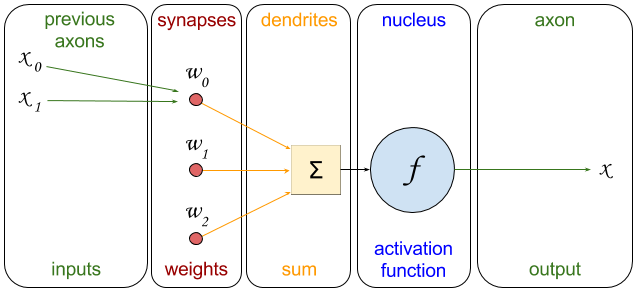
\includegraphics[width=0.8\linewidth,center]{images/part1/neuron_schema.png}
  \caption{Mathematical representation of a neuron used in Neural Networks}\textbf{
  \label{fig:part1:neuron_schema}}
\end{figure}

Then, as its name implies, a neural network is a network composed of neurons, connected in some defined ways, often organized in few layers, and with a specific activation function (sigmoid, tanh, ReLU, ...). Most of the neural networks follow a feed-forward supervised learning method : the main idea of this learning consists in giving an information as input, doing a forward pass until the last neurons, then comparing the output with the expected one and, finally, according to this comparison, doing a backward pass through the network to its beginning by changing the weights of each neuron to adapt them to the expected result. After some iterations, the model learn perfectly how to process the given input. The interest is to give many various data to allow the system to understand a concept within all the data and to reuse it on an unknown information. As an example, if we provide hundreds images of faces to a neural network, make it learn if these faces are males or females, the system should also be able to detect the sex of a new (unknown) face at the end of the learning.


\subsection{The special case of Convolutional Neural Network} \label{1:overview:special_case}
Neural networks used to use affine transformations, that means that they get a vector as input, and they multiplied it with a matrix (depending on the current layer) to produce an output. Main point is that it can be applied to many kind of input, such as sound, multiple features, or images, whatever their dimensionality, because they all are stored as multi-dimensional arrays, so then they can be converted into a vector of data. But one problem is that, in our case, the order of the data may matters (each pixel have a specific location in an image ; a sound has to be listened from its beginning to its end), and our data also have one channel axis used to access different characteristics of it (RGB channels for the image ; left and right channels for audio data). These two properties are not preserved with the affine transformations : they treated all the axis in the same way and the topological information is not taken into account.. To deal with this kind of data, CNN use linear transformation (more specifically discrete convolution), which preserves the notion of ordering and gave their name to the Convolutional Neural Networks.

Usually, each Convolutional Neural Network is mainly composed of the two following layers.
\begin{itemize}
\item[-] \textbf{Convolutional layers} with the following characteristics :
\begin{table}[ht!]
  \centering
  \resizebox{\textwidth}{!}{
    \begin{tabular}{l|p{10cm}}
    \toprule
    $i_j$    & size of the input along axis $j$		 \\
	$D$      & depth of the input					 \\
	$K$		 & number of filters (or kernels)		 \\
	$k_j$    & size of the kernel along axis $j$      \\
    $s_j$	 & stride : distance between two consecutive positions of the kernel along axis $j$ \\
	$p_j$   	 & zero-padding : number of zeros concatenated at the beginning and at the and of an axis along axis $j$	 \\
	$d$		 & dilation, introduced by~\cite{YU15}, permit filters to have spaces between each cell. It is, by default, set to zero.	 \\
    \bottomrule
    \end{tabular}%
  }
  \caption{Convolutional layer characteristics}
\end{table}%

  The input data, for example a greyscale image (dimension 2, size 5x5x1) is processed by a set of small learnable filters kernel. Indeed, every single neuron of the convolutional layer volume is connected to a small region ($k_x$x$k_y$x$D$) in the input volume, and sees its weights evolve during the learning. The figure~\ref{fig:part1:imagenet_weights} shows an example of the final filters that a system may learn. These layers drastically increase the number of features, which turns to be one of the main problematic for some architectures~\cite{SZEG15}.
\begin{figure}[ht!]
  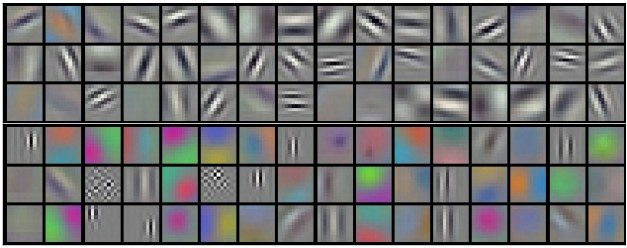
\includegraphics[width=0.8\linewidth,center]{images/part1/imagenet_weights.jpeg}
  \caption{Example of filters learned by Krizhevsky et al~\cite{KRIZ12}.}\textbf{
  \label{fig:part1:imagenet_weights}}
\end{figure} \\
  The output of the layer would be a volume of size $W'$x$H'$x$D'$ with :
  \begin{itemize}
  \item $W' = \frac{i_0 - k_0 + 2p_0}{s_0} + 1$
  \item $H' = \frac{i_1 - k_1 + 2p_1}{s_1} + 1$
  \item $D' = K$
  \item $k_0 * k_1 * D$ different weights per filter
  \end{itemize}

\item[-] \textbf{Pooling layers} with the following few characteristics :
\begin{table}[ht!]
  \centering
  \resizebox{\textwidth}{!}{
    \begin{tabular}{l|p{10cm}}
    \toprule
    $i_j$    & size of the input along axis $j$		 \\
	$D$      & depth of the input 					 \\
	$k_j$    & size of the pooling window along axis $j$      \\
    $s_j$	 & stride : distance between two consecutive positions of the pooling window along axis $j$ \\
    \bottomrule
    \end{tabular}%
  }
  \caption{Pooling layer characteristics}
\end{table}%

  These layers permit to reduce the number of characteristics in the network by reducing the size of the features. It is a simple operation, simply doing the same as discrete convolution but replace linear combination by some other function (usually max, or mean, but some other can be applied~\cite{BOUR10, COMA02, SAXE11}). \\
  The output of the layer would be a volume of size $W'$x$H'$x$D'$ with :
  \begin{itemize}
  \item $W' = \frac{i_0 - k_0}{s_0} + 1$
  \item $H' = \frac{i_1 - k_1}{s_1} + 1$
  \item $D' = D$
  \item $k_0 * k_1 * D$ different weights per filter
  \end{itemize}
  New architectures tend to reduce the number of pooling layers to zero~\cite{SPRI14} by using, instead of them, convolutional layers with larger strides.
\end{itemize}


\subsection{How to play with them ?} \label{1:overview:play}
Few things should be taken in consideration while creating a Deep Learning architecture :

First, the input layer, that handles the data. The size of the given data have to be divided by 2 few times. Indeed, pooling layers used to divide the size of the data while increasing its depth (number of features).

About the layers, the convolutional layers should use small filters if they want to keep a relevant information (often 3x3, and 5x5 is mostly the biggest acceptable size). They also have to use a small stride (stride of 1 is often the best solution) because it permits to cross the whole data, also keeping the neighbourhood notion. Then, the zero-padding should be selected according to the expected output size, following the formulas given in section~\ref{1:overview:special_case}, it is mandatory, here, to avoid altering the spatial dimensions of the input.

Also, the pool layers are used to downsample the data, and they mostly use max-pooling (extracts the biggest element in the pool window) with a pool window of size 2x2 and a stride of 2x2. These settings permit to cross each element of the whole data only once, and it reduces the size of all the features by 2. Larger pool windows usually decrease the global performance of the system, because they are to aggressive (alter the main information).

Finally, some parameters can be modified considering the memory constraints of the GPU. As en example, filtering a 224x224x3 image with three 3x3 convolutional layers (64 filters each and zero-padding of 1x1) would lead to around 10 million activations.. A solution is, then, to reduce the size of the input data, or to reconsider the deep learning architecture for reducing the total number of parameters.


\subsection{The upscaling problem}
CNNs provide a linear output : usually a vector of data. More specifically, a DL architecture for classification use to return one probability per class, corresponding to the main object present in the image (in case of object recognition). This method is not enough for semantic segmentation, because we actually want these probabilities for each pixel of the image. To do this, we need to upsample the vector of data into an array of vectors, using the features of the network.

This is a challenging task because the features obtained by the convolutional layers are difficult to interpret. Fortunately, one of the characteristic of the convolutional layer is that it preserves the localization of the features, and so, it preserves the general way the image is organized. Few methods exist to upsample a map of features, and some of them will be described in the following sections.




\section{Comparison of many different architectures} \label{1:comparison}
\subsection{CNN for classification} \label{1:comparison:classification}
\subsubsection{LeNet} Introduced by Yann LeCun in 1990's~\cite{LECU98}, LeNet is known as the first CNN that was able to provide good results. It is mainly used for patterns recognition, such as handwritten and machine-printed characters. The LeNet architecture only have three convolutional layers, and use, at its end, a fully connected layer to get the appropriate class from all the features. Its simple architecture involves a low number of parameters (only 0.43M).

\subsubsection{AlexNet} Introduced by Alex Krizhevsky in 2012~\cite{KRIZ12}, AlexNet popularized CNN in computer vision by winning, by far, the ILSVRC challenge in 2012~\cite{RUSS15}. Its architecture is very similar to LeNet's, except that it is deeper and introduced series of convolutional layers (usually, each convolutional layers were followed by pooling layers). It has 5 convolutional layers, ends with three fully connected layers, and produces a super high number of parameters (60M vs less than 1M for LeNet).

\subsubsection{VGGNet} Introduced by Karen Simonyan in 2014~\cite{SIMO14}, VGGNet has two different available architectures : one with 16 convolutional layers, and an other one with 19 convolutional layers. The main goal of this work was to prove that the depth of a network (16 or 19 layers instead of 5 in AlexNet) does affect its accuracy. These very deep models conduct to a huge amount of parameters that did not suit with any regular GPU. To fix this, the authors used very small filters in all the convolutional layers (3x3, stride 1x1), resulting to a final number of 138M parameters. This number is still huge, but the model proves its efficiency by winning the 2014 ILSVRC Challenge.

\subsubsection{GoogleNet} Introduced by Christian Szegedy (Google) in 2014~\cite{SZEG15}, GoogleNet proposes a new module (Inception module) that increases the depth and width of a network while keeping its number of parameters constant. They finally proposed a deep network (22 convolutional layers) that used only 6.8M parameters (instead of 60M for AlexNet, which has much less convolutional layers). The main beneficial aspect of this architecture is that it aggregates data information at various scales. This should intuitively save features mostly according to their context than to their identities.

\subsubsection{ResNet} Introduced by Kaiming He in 2015~\cite{HE16}, the ResNet architecture introduced residual learning by adding some skip connections to the architecture. Each shortcut connection skips one or more layers and performs an identity mapping that is added to the output of the regular stacked layers. This method aims to reduce overfitting and architecture complexity by using another way to store the weights of each layer : instead of storing all the information, they propose to save the difference between the expected underlying map with the output map (get from the stacked layers). To the extreme, if our map fit perfectly with the expected result, we would just have to set it to zero instead of adapting it to make it fully suitable to the expected map. Moreover, if the shortcut connection skips more than one layer, it permits to store the information for all of these layers in one single map, which permits to considerably increase the depth of the network. They propose three variants of this architecture : ResNet-50, ResNet-101 and ResNet-152 (they respectively have 50, 101, and 152 layers). The ResNet-152 architecture won the 1\textsuperscript{st} place on ILSVRC 2015 and only have around 2.3 parameters, despite its depth. This number of parameters is actually 30 times lower than AlexNet, and it is 30 times bigger than AlexNet.


\subsection{CNN for semantic segmentation} \label{1:comparison:segmentation}
Convolutional Neural Networks doing upscaling methods are finally really similar except that they add an upscaling method.
\subsubsection{SegNet} Introduced by Vijay Badrinarayanan in 2015~\cite{BADR15}, SegNet reuses the 13 first layers of the VGG16 network and, then, proposes an upscaling method to do semantic segmentation. The main idea is to keep the indices of the max-pooling layers (it saves the selected max element for each window pool translation in each pooling layer) and, then, to use it for performing non linear upsampling (which increase the size of the image instead of reducing it as usual pooling layer do). This architecture is mainly used for road-scenes understanding, permitting to know with precision where are located pedestrians, cars, building, etc. \\
Its architecture is divided in two main parts : the encoder, which corresponds to the 13\textsuperscript{th} first convolutional layers of VGG16, and the decoder, which is composed of the same, but reversed, layers, which used to upsample the image to a coherent output. The schema~\ref{fig:part1:segnet_architecture} illustrates the SegNet architecture.

\begin{figure}[ht!]
  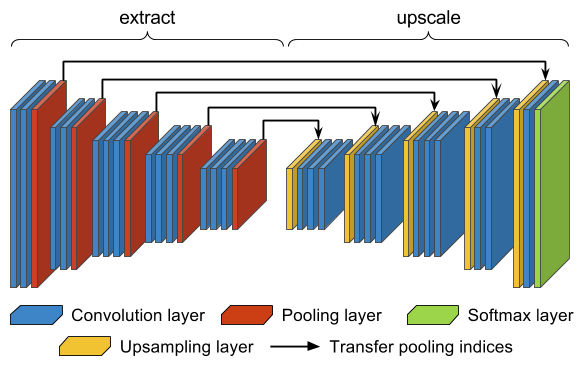
\includegraphics[width=0.8\linewidth,center]{images/part1/segnet_architecture.png}
  \caption{Architecture of SegNet}\textbf{
  \label{fig:part1:segnet_architecture}}
\end{figure}

\subsubsection{FCN} Introduced by Jon Long in 2015~\cite{LONG15}, three upsampling models are proposed : the 32s one, the 16s', and the 8s'. All of these can be applied to few classification methods, but they mainly proved their efficiency on VGG16 and GoogleNet (AlexNet is also suitable, but don't provide any comparable accuracy level). About VGG, they simply took the 13 first convolutional layers of VGG16 (as SegNet does), and converted the last layers into deconvolution layers, which are similar to convolutional layers except that they upsample the size of the features instead of decreasing them. About GoogleNet, they did the same by replacing the final loss layer by deconvolution layers. Both of them ends with a 1x1 convolution with a specific channel dimension (corresponding to the number of classes in the dataset), permitting the prediction. The FCN-16s version is the same, but also adds an other connection between the last convolutional layer to the first upsampling layer, permitting to add their outputs and compute more specific results. Finally, the FCN-8s version is similar to FCN-16, except that it adds two connections between the two last convolutional layers and the two first upsampling layers. The schema~\ref{fig:part1:fcn8_architecture} illustrates the architecture of FCN-8, and a comparison of these three variants (FCN-32, 16, and 8) is proposed in appendices~\ref{fig:appendices:fcns_architecture}.

\begin{figure}[ht!]
  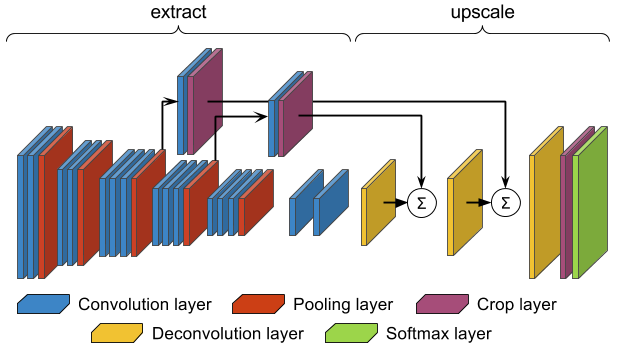
\includegraphics[width=0.9\linewidth,center]{images/part1/fcn8_architecture}
  \caption{Architecture of FCN-8}\textbf{
  \label{fig:part1:fcn8_architecture}}
\end{figure}


\subsubsection{FCN-32-ResNet and FCN-16-ResNet} As we saw in the previous section (~\ref{1:comparison:classification}), ResNet seems to be a very good architecture for classification, so we decided to try it for pixel-wise labelling by adding the upsampling methods of FCN. We propose here, two variants : one with the upsampling method of FCN-32, as shown in the schema~\ref{fig:part1:fcn-resnets:32}, and an other one with the upsampling method of FCN-16, as shown in the schema~\ref{fig:part1:fcn-resnets:16}. Both of these figures are done with the ResNet-50 architecture, to improve the visibility, but we created, for both of them, the three variants (50, 101, and 152 layers).

\begin{figure}[ht!]
\centering
\begin{subfigure}{.9\textwidth}
  \centering
  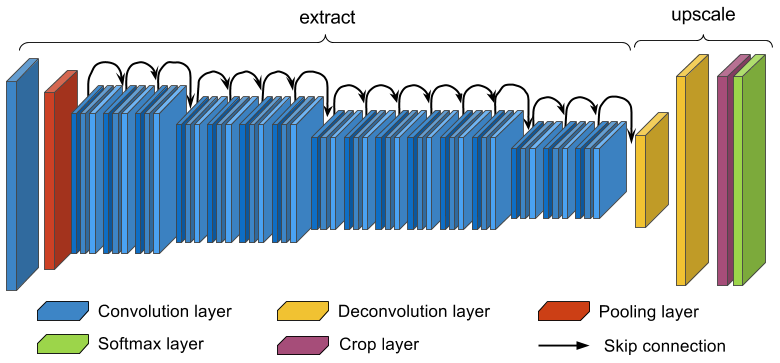
\includegraphics[width=0.9\linewidth,center]{images/part1/fcn32_resnet_architecture.png}
  \caption{Architecture of FCN-32-ResNet-50}
\end{subfigure}%
\label{fig:part1:fcn-resnets:32}
\\
\begin{subfigure}{\textwidth}
  \centering
  \includegraphics[width=\linewidth,center]{images/part1/fcn16_resnet_architecture.png}
  \caption{Architecture of FCN-16-ResNet-50}
\end{subfigure}
\label{fig:part1:fcn-resnets:16}
\caption{FCN-xx-ResNet-50}
\end{figure}
\label{fig:part1:fcn-resnets}

\subsubsection{CRF-RNN} Introduced by Shuai Zeng, in 2015~\cite{ZHEN15}, this network, called CRF-RNN (Conditional Random Fields - Recurrent Neural Network), aims to improve the accuracy of delineations for CNN. It proposes to learn some other features relative to the context, permitting a post-processing step, at the end of a network, that improves the accuracy of the delineations using probabilistic-based formula. Basically, it checks, for each pixel, if its labelling is coherent according to its neighbourhood, considering the usual neighbourhood of this kind of label learnt during the training. This end-to-end architecture works well, but have two big limitations : first, it takes a long time to process and, secondly, it is not available as easily as the other architectures on Deep Learning frameworks. So it actually requires to code a big part of it by ourself, and to reconsider it to make it suitable to our own architectures.

\subsection{Comparison of these architectures} \label{1:comparison:comparison}
The first thing to note is about the classification models : it is the revolution of depth. The schema~\ref{fig:part1:comparison_archi_classification} shows that the models, years after years, improve their depth with their accuracies. Also it has been noticed~\cite{SIMO14, SZEG15, HE16} that the depth of a network involves a biggest number of parameters to learn, and that this one could be a problem with our GPUs capacities. Considering this, many recent works try to decrease this number over these last years.

\begin{figure}[ht!]
  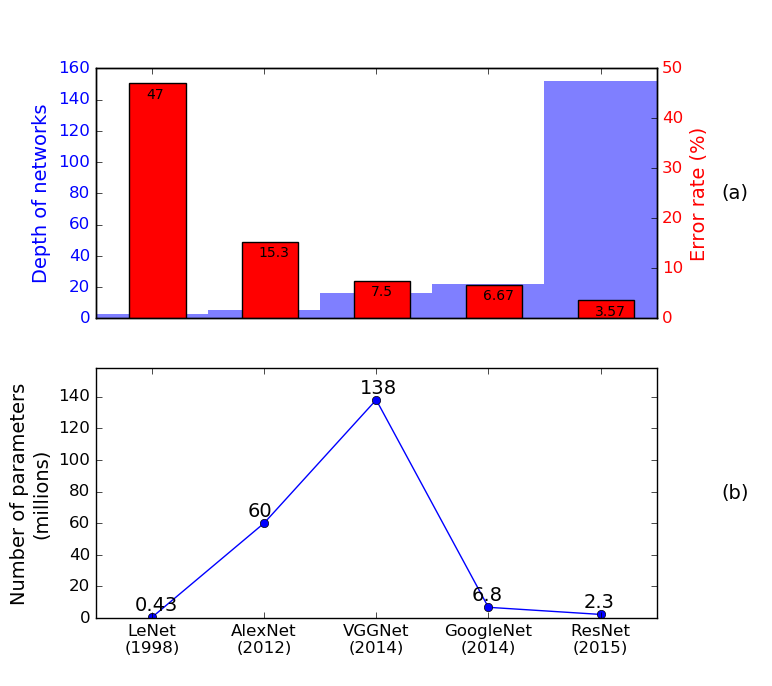
\includegraphics[width=\linewidth,center]{images/part1/comparison_archi_classification.png}
  \caption{Revolution of depth throught classification architectures}\textbf{
  \label{fig:part1:comparison_archi_classification}}
\end{figure}

The other main point from the architecture is about the upscaling methods. It doesn't exist a huge variety of them, but they are actually quite different. If SegNet reuses the encoding step, FCN completely ignores it and is implementable end-to-end (just as a patch, at the end of a network). CRF is also really different because more based on image post-processing.




         \pagebreak
  \chapter{Flexibility between various datasets}

To build a Deep Learning system that works for some data, it needs to learn how to process them. To do that, we have to make it learn correct weights (for each of its layers) by doing supervised learning with a given dataset. But the characteristics of the dataset will obviously have a huge influence on the learning, so we have to be careful while choosing and/or building the dataset. We also will see how to deal efficiently with different dataset with one single DL system. In this section, we will focus ourselves on datasets composed of pictures, but we have to keep in mind that we also can work with other kind of data.



\section{A wide range of datasets}
\subsection{Many characteristics}
It exists many datasets for computer vision, and they all differ by some given characteristics :
\begin{itemize}
\item Their context : A dataset can be done with many different contexts, or with only a specific one. Indeed, it can be built with multiple kind of pictures : indoor, outdoor, by night, aerial, alone-object focus... A dataset with multiple kind of pictures is more difficult to learn by the system because it would involve to learn a lot of features for a lot of different objects and to understand that each of them can also have multiple instances (by night, reverse, half-hidden, ...). On the other hand, if we have a dataset composed in integrity by cat pictures, the system will learn something really specific (cat recognition) and won't be flexible to other images.
\item Their number of classes : Most of the pictures of our dataset would represent several objects and not only one defined object. Indeed, even a simple cat picture would have a complex background (plant, ground, wall, kennel, ...) and we have to define if we want to extract some information on this. Most of the datasets have a small number of classes but the biggest ones can grew up to few thousands classes.
\item Their way to segment the pictures : the way to segment the image is different, it depends on the future application of the system. For example, if we want to build a system able to distinguish pictures of cats and dogs, we won't need to segment them, a simple label corresponding to the appropriate class attached to the picture would be enough. If we also want to locate the pet, we should then attach the label with the location. The table~\ref{fig:part2:segmentation_comparison} shows three examples of segmentation, including pixel-wise labelling.

\begin{figure}[ht!]
  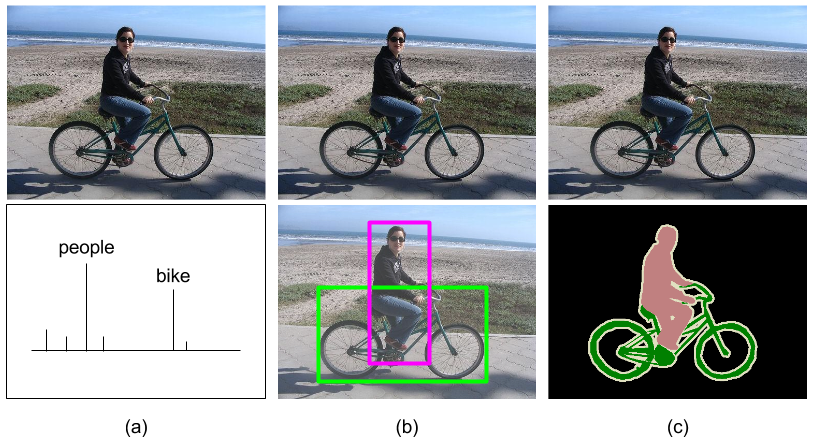
\includegraphics[width=\linewidth,center]{images/part2/segmentation_comparison.png}
  \caption{Different segmentation kind}\textbf{
  \label{fig:part2:segmentation_comparison}}
\end{figure}

\end{itemize}


\subsection{A quick state of the art} \label{2:datasets:soa}
Basically, few dataset are famous in computer vision, here is a non-exhaustive list of them, and a visual example for each of them is also provided as appendix~\ref{fig:appendices:datasets_comparison} :
\subsubsection{MNIST} This database contains 70.000 handwritten digits which have been size-normalized and centered in a fixed-size image. The works of Yann LeCun~\cite{LECU95, LECU98}, one of the father of Deep Learning, are based on this dataset and allowed a system to convert a written text into a typing text. Each image has a single label, corresponding to its appropriate letter or number.
\subsubsection{ImageNet} One of the biggest dataset currently used for Deep Learning system, it is composed by more than 14 million images, representing situations in the world without limitation (group of people, table, dog in kennel, candy shop, ...). These images are labelled according to more than 21 thousand classes, divided into 27 high level categories (fruit, person, vehicle, ...). Every single image have one label, corresponding to the class of the main object in the picture, and about one million of them also have a bounding box annotations (the objects in the images are bounded by a square). Most of the architectures are tested on ImageNet because of its size, and it finally turns into a really famous challenge (ILSVRC Challenge~\cite{RUSS15}).
\subsubsection{Pascal VOC} An other famous image dataset, pretty similar to ImageNet by its diversity, is the Pasxal VOC's. The main difference is the labelling methods : Pascal VOC proposes a semantic segmentation of its images, where each pixel of each label is labelled as belonging to one class. The other main difference is, obviously, its size (it is much longer to segment an image than simply label it), so Pascal VOC 2012 has almost 12 thousand images segmenting 21 different classes. Also, the images don't respect any size normalization. This dataset is the most famous in the semantic segmentation field, and also have its own challenge~\cite{EVER10}.
\subsubsection{SBD} The Berkeley Segmentation Dataset~\cite{MART01} is similar to Pascal VOC and ImageNet by the diversity of its images. It is composed of 12 thousand images which all have a boundary segmentation. This kind of segmentation can be used for pixel wise labelling, improving the accuracy of the boundaries.
\subsubsection{MS COCO} This dataset, from Microsoft~\cite{LIN14}, is less famous than the previous ones, but also provides a large dataset with partial semantic segmentation (for each image, the labelling contains at most 10 instance per given categories). For images containing a highest number of instances (such as crowds for people, car parks for cars, forests for trees, ...) areas are notated as "crowd". The dataset is large, composed of 300.000 images, which are divided in 80 different categories.
\subsubsection{CamVid} The CamVid dataset~\cite{BROS09} is not famous at all in the Deep Learning field, but we cite it here because it is, in a way, really close to the dataset we are going to create with aerial-views. Indeed, it is composed by images captured from the perspective of a driving automobile. All of them have a complete semantic segmentation, and the background class ("unknown" class) has a really small place in the dataset. This dataset is composed of over 700 images, divided in 32 semantic high level classes, covering most of a driving-based view.


\section{Focus on aerial views}
\subsection{Many questions to answer}
As we saw previously, we have to answer to many questions while creating a dataset. Here is a list of few of them, focusing on the aerial views problem.

First, we have to define the context. In the case of this project, we want some aerial-views, so all the images are going to be taken from the perspective of a drone. Few questions still remain there, like the height of the drone, because the shape of objects drastically changes with the point of view. Also, we have to wonder about the angle of the camera : it can be oriented to the ground, or a bit elevated (oblique view). Finally, it is also important to decide where does the drone will fly. Indeed, if it flies only above fields, our system would not be able to segment buildings, because he would see them for the first time. Of course, a single dataset can merge few of these characteristics (such as views from 50m and 70m), but it may affect the learning if the dataset is too small.

Secondly, the labelling type is important, but also quite obvious for this project. The aim of the project is to offer a detailed information of its visual environment to the drone in real time, so we want the most-detailed level of information. The pixel-wise segmentation (defining one single class per pixel) is a good way to build this information. We also saw the example of SBD in section~\ref{2:datasets:soa} that only labels boundaries for each image. It also can be interesting for our project, but the efficiency of this kind of segmentation has not been proven yet and it is simple to generate this boundary from the pixel-wise segmentation (the reciprocal is not true).

Thirdly, and maybe one of the most important point, we have to define the number of classes. Most of aerial views would display some common objects, such as building, pedestrians, cars, pavements... but also some uncommon objects like train tracks, trucks, sport areas... A solution is to analyse each image of our dataset before doing segmentation, to note every single objects present in it, and to deduce the final number of classes. The problem is that it would involve a too large number of classes with some of them really rare, and it may disturbs the learning. An other solution is to resume all of these classes into few big categories (pavement, road, car parks all labelled as "paved ground" for example), but it also should depend on the final application of the system : do we need to distinguish car parks ? Or recognizing it as a paved ground is enough ?

Fourthly, the precision of the dataset. Indeed, what would be the size of the image, and the level of detail ? If we saw a pedestrian on a few amount of pixel, should we consider him ? Moreover, the size of the image should respect the computation constraints of the GPU (it also depends on the memory required by the architecture) and we should also take in consideration the real-time notion.

Fifthly, the size of the dataset. A biggest dataset would offer a better accuracy and flexibility if its diversity increases with its size. But building a big dataset takes a long time, and involved the work of many people~\cite{LIN14}, so we have to determine what can be the most interesting alternative.


\subsection{What we chose to do}
We chose to build two different small datasets. Indeed, it is more interesting to run our experiments on two different sets for testing the reproducibility of them, and also to play with our architectures on both of them, to see how it affects the learning. For both datasets, we chose to use the same general classes.
\begin{enumerate}
\item The first dataset is taken from the swiss company senseFly\footnote{sensefly.com/drones/example-datasets} database. We used the dataset \textit{senseFly HGsite} and did pixel-wise segmentation on 100 images. On this dataset, the drone only flies above one area with industrial areas, fields, and residential districts. Each image has a size of 4608x3456, is taken at 88m of altitude, and has a view pointing to the ground (90 degrees).
\item The second dataset has been done by our own drone, in Okutama (Japan), and the images are taken from two different areas : around a baseball field and around a highschool. These two areas present some industrial, residential, sport areas and some forests. Each of the 28 images has a size of 3840x2160, is taken at 90m of altitude, and has, as above, a view pointing to the ground (90 degrees).
\end{enumerate}
For both of them, we chose to segment the following 10 classes : background, structures, building, pavement, non-paved ground, train tracks, plants, vehicles, water and people. The figure~\ref{fig:datasets_example} shows an example of this two datasets.

\begin{figure}[ht!]
\centering
\begin{subfigure}{.5\textwidth}
  \centering
  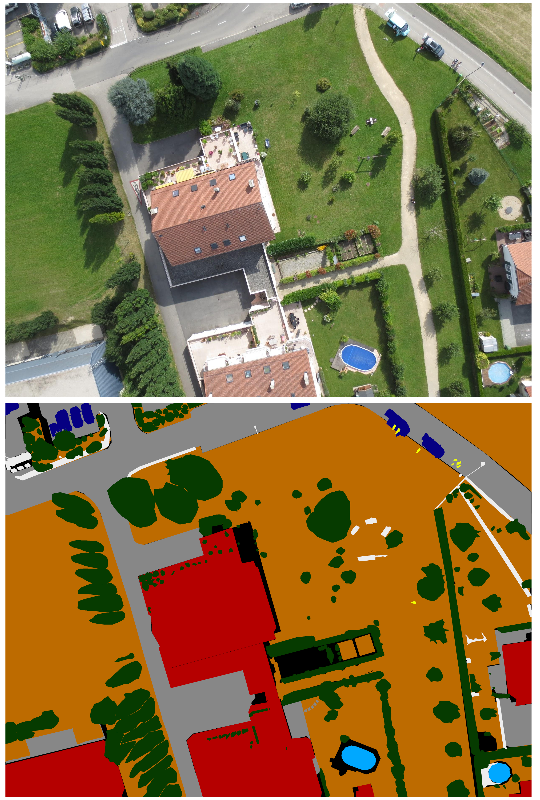
\includegraphics[height=7cm]{images/part2/swiss_example.png}
  \caption{Swiss dataset}
  \label{fig:part2:swiss_example}
\end{subfigure}%
\begin{subfigure}{.5\textwidth}
  \centering
  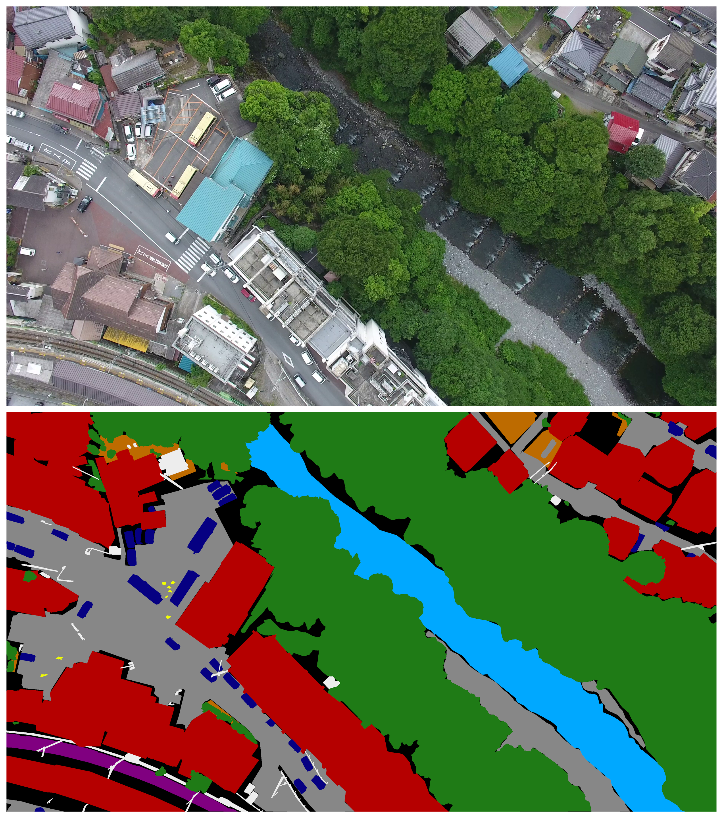
\includegraphics[height=7cm]{images/part2/oku_example.png}
  \caption{Okutama dataset}
  \label{fig:part2:oku_example}
\end{subfigure}
\caption{Datasets created}
\label{fig:datasets_example}
\end{figure}



\section{Deep Transfer Learning}
\subsection{Why do we have to use DTL ?}
Considering that we have two different small datasets, for example one with aerial views with an oblique point of view, and an other one with a ground-oriented point of view. Then, we want our system to learn both of these features (learn that a tree can look like either a green circle or a more complex shape green oval overcome by a brown line, the trunk). The most intuitive idea is, then, to do one single big dataset with all the images and to give this to the system, but it finally may affect the learning because the system won't see a sufficient amount of images with both of these characteristics to understand their differences and assimilate them as features of the same object. In that case, a solution could be to train both of these networks separately and, then to merge their learning as a single one.

An other problem can be pointed out : if we have two dataset, one large dataset with aerial views, permitting to our system to learn really efficiently the features of all the main objects, and an other small dataset with the same images, but with some disaster situations (fires, collapses, ...). We want to keep the accuracy of our system while it learns the big dataset, but also make it able to detect new situations on known classes (the system knows what a building looks like, but won't recognize it if it is on fire). Then, we also can't merge both datasets because there is too few images with buildings on fire, it won't learn it. Then, a solution is to learn, first, the big dataset and, then, to complete our learning slowly with the small one, modifying it really carefully.


\subsection{A brief overview}
In practise, training a network from scratch (from nothing, with a random initialization) is really long, and may provide incomplete results because of an insufficient size of the dataset. Usually, it is more efficient to transfer the weights learnt from a very large dataset (such as ImageNet that has almost 1.2M images), even if our dataset is significantly different. The main idea of Deep Transfer Learning is to transfer some knowledge of a system to an other system. Both of these networks may have learnt features from different datasets, and the merging of both of these learning permits to increase the global accuracy over them. In a general way, we have the "source" dataset $D_s$, used for training an architecture $A_s$, that provides some results $W_s$. We, now, want to transfer what we have learnt with the "source" network into the target architecture $A_t$ (learning from dataset $D_t$, and would give the weights $W_t$). For all the Deep Transfer Learning methods, $A_s$ and $A_t$ must be really similar (at least their basal).

\subsubsection{Feature extractor}
The first transfer method is actually, really simple, it only consists in replacing the last fully connected layer in the source architecture by an other one. Then, the architecture will still keep its learning, but will provide different outputs. For example, a CNN pretrained on ImageNet will give an output for one thousand classes. Changing the number of outputs on the last layer and retrain it permits us to reuse the weights of ImageNet on an other, smaller, dataset. This method only works when $D_s$ and $D_t$ are really similar, and $A_s$ and $A_t$ are, there, the same.

\subsubsection{Finetuning}
Finetuning is a really well-known transfer learning method in Deep Learning. It actually consists in replacing, not only the last layer, but also some other layers, a bit deeper in the architecture. The main concept is to keep the basal of the network, and to modify the weights of the other layers during backpropagation. This method has been introduced when we realized that the first layers usually contain more generic features that could be useful even in different architectures. On the other hand, latest layers are more specifics, and may be changed if we want to adapt our learning to a different dataset. The figure~\ref{fig:part2:finetuning} shows an example of a finetuned architecture, showing that some layers are like "frozen" (layers in blue), keeping the weights from the source architecture during the learning. Then, during the backward pass, the weights of the latest layers (white layers) would be the only ones to modify.

\begin{figure}[ht!]
  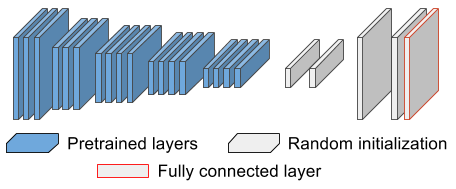
\includegraphics[width=0.8\linewidth,center]{images/part2/finetuning.png}
  \caption{Finetuning process}\textbf{
  \label{fig:part2:finetuning}}
\end{figure}

Actually, considering our small datasets, it is mandatory to use finetuning method for all of our experiments, a training from scratch would not be efficient. As an example, the curve~\ref{fig:part2:loss_bad} represents the loss function (function we try to minimize during the training, corresponding to a proportional inverse of the accuracy) we get while training from scratch. On the other hand, the curve~\ref{fig:part2:loss_good} is the one using finetuning.

\begin{figure}[ht!]
\centering
\begin{subfigure}{.5\textwidth}
  \centering
  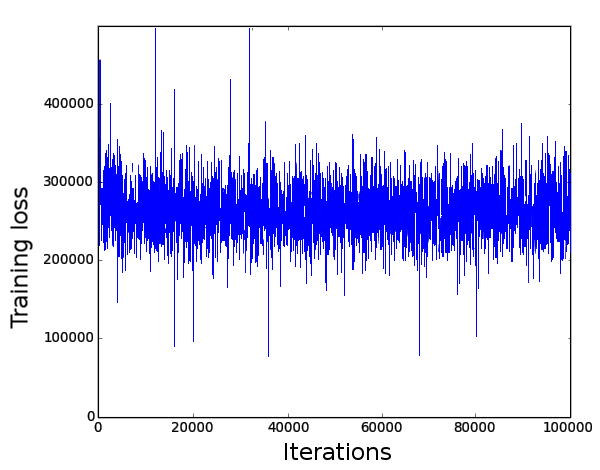
\includegraphics[width=0.9\linewidth]{images/part2/loss_bad.png}
  \caption{Loss without weight initialization}
  \label{fig:part2:loss_bad}
\end{subfigure}%
\begin{subfigure}{.5\textwidth}
  \centering
  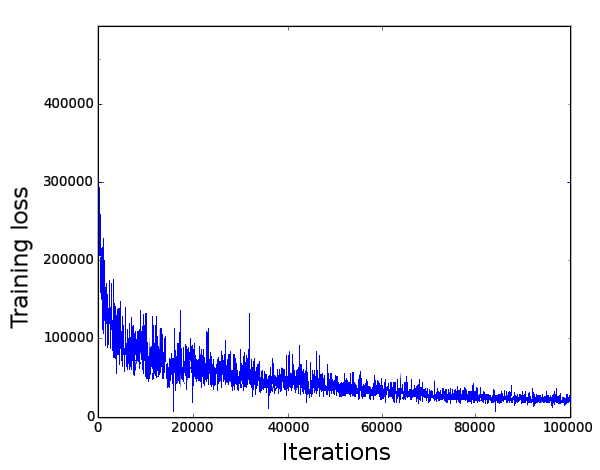
\includegraphics[width=0.9\linewidth]{images/part2/loss_good.png}
  \caption{Loss with weight initialization}
  \label{fig:part2:loss_good}
\end{subfigure}
\caption{Comparison of losses with or without initializations}
\label{fig:loss_comparison}
\end{figure}


\subsubsection{Multi-Source}
The multi-source transfer learning method~\cite{KAND16} can be more efficient, considering our project. Indeed, it has, as goal, to improve the general accuracy performed by one architecture on two different datasets. The main idea is to learn weights from the source dataset, then to finetune them with the target dataset, and to repeat these two operations for few cycles. Doing this, the learning of the source dataset is preserved, but also includes the features from the target dataset. This method improves the global accuracy (average of accuracies over both datasets), and also may improve the accuracy of the source dataset if it has some features close to the target. In our case, we have two datasets with aerial views, so the features from one dataset may help the architecture on the other one. This method can also be extended on more than two datasets, and also can be improved by playing on some parameters (such as decreasing the learning rate through the cycle). The figure~\ref{fig:part2:multisource} displays the functioning of Multi-Source over two dataset.

\todo{to clarify}
\begin{figure}[ht!]
  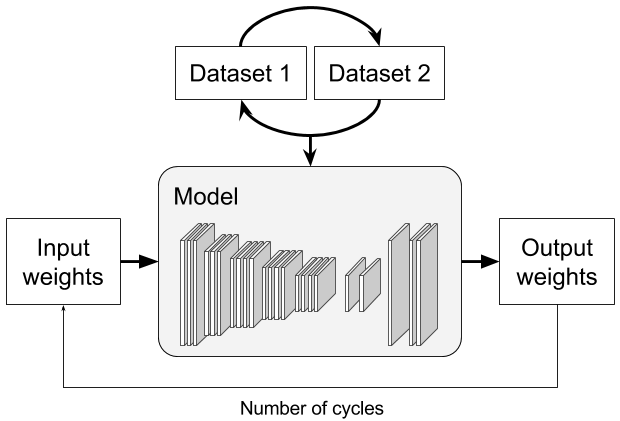
\includegraphics[width=0.8\linewidth,center]{images/part2/multisource.png}
  \caption{Multisource process between two datasets}\textbf{
  \label{fig:part2:multisource}}
\end{figure}





         \pagebreak
  \chapter{Methodology}


In the previous parts, we saw that many architectures exist in computer vision and we also defined our two datasets for this project. We now have to define the tools we are going to use to implement everything, and the research methodology for detecting the best model and learning method for our project.


\section{The tools used}
\subsection{The Caffe framework}
As saw in section~\ref{1:overview}, every convolutional network respect some characteristics (composed of the same kind of layers, same learning methods, same way to do the forward / backward passes, ...), so some frameworks propose to simplify their implementation. It is quite mandatory to use one of them because they permit to avoid a long implementation time, and they usually are well-structured, increasing the speed of the computation (easy use of GPUs, compact use of DL libraries, etc).

At this point, the necessity of the framework is obvious, but one problem remains : which one ? Indeed, it exists a lot of variants (Caffe, Torch, Theano, openNLP, dmc, CNTK, ...) and all of them have some different characteristics, so we have to chose the best according to our project. In our case, we have few requirements that may influence our choice :
\begin{itemize}
\item The number of models available on it : indeed, we want to compare few architectures, so we need to compare all of them on our own data. To do this, it is easier if they are already implemented in the framework, or if everything is done to simplify their implementation.
\item The speed of the framework : one of the main point of our project is that we want to implement this framework (handling our DL architecture) in a drone to make it able to process its camera vision in semi-real-time. Considering this, the speed is really important if we want to keep the "real-time" notion.
\item The flexibility of the framework : some frameworks are specifics to CNN, or to RNN. In our case, we mainly want it to be flexible to CNN, and, if possible, able to handle new models easily. Indeed, if we want to do some deep changes on our architecture, the framework should be flexible to some unknown kind of architectures.
\item The global structure of the framework : first, its documentation, then, its language (are we able to code it), and the genericness of the framework over DL methods.
\end{itemize}

We compared all of these points on five different framework, considered as the most famous frameworks in Deep Learning nowadays, and resumed all the data into the table~\ref{appendices:frameworks_comparison}, in the appendices.

Considering this, Caffe and Torch appear as the best solutions for our project. Between both of them, Caffe is most easy to use, has a huge community and is mainly usable without writing a single line of code because of its structure. Torch seems more complicated (require to write some code in Lua), but also more flexible to new layers / new architectures and it also has a lot of pretrained models. On the other hand, Torch is mainly useful if we want to create really specific architectures (new kind of data processing, new layers, ...) and, in our case, we mostly want to reuse existing methods to compare them and, then, improve them if possible. Considering this, Caffe seems to be the most suitable framework to use for now.


\subsection{A framework for the DTL}
Caffe is a good framework for handling the Deep Learning architecture, it allows to load and to run it efficiently (within a good processing time). But for our project, we need to compare many different architectures, and we also would need to do some deep transfer learning. Most of them can be done using only Caffe, but it is not intuitive, not efficient (it breaks explicitly the trainings into sub-training) and we may be confused between all our experiments.

To deal with these issues, we decided to create our own framework, mostly focused on the deep transfer learning methods, that includes Caffe. The schema~\ref{fig:part3:dtl_framework_architecture} shows the architecture of both frameworks linked together. Globally, it takes, as input, a prototxt file (format introduced by the google protobuf library~\footnote{developers.google.com/protocol-buffers}), listing the transfer learning methods to use. A learning method is composed of many stages those actually define a training method \textit{via} their own prototxt, defining the architecture (train.prototxt) and its parameters (solver.prototxt).
In a more general way, the framework took some weights as input, and uses them for the first stage of the DTL method (fine-tuning). Once the training is over, we get the new weights, and use them as input the next stage. The trainings can be processed in different orders, recursively, with a decreasing learning rate, etc...

\todo{bold the "for" and "in"}
\todo{add the parameters in the stages}
\begin{figure}[ht!]
  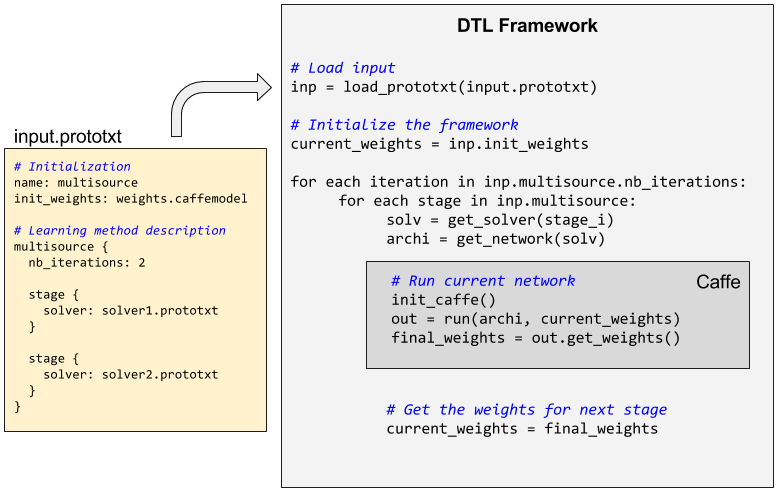
\includegraphics[width=\linewidth,center]{images/part3/dtl_framework_architecture.png}
  \caption{Architecture of the Deep Transfer Learning framework}\textbf{
  \label{fig:part3:dtl_framework_architecture}}
\end{figure}


\subsection{The metrics used} \label{3:tools:metrics}
For evaluating efficiently the accuracy of a model, we need to define a good evaluation measure. In our case, we are interested by semantic segmentation (pixel-wise labelling), so there are actually a lot of metrics those already exist in that field. It is complicated to define if the algorithm has made a "good job" because all of them have different requirements and goals : some applications does not need a perfect segmentation (with a precise delineation of the contours), and so, some algorithms can be considered efficient if they segment the images into uneven blobs as long as they classify them well.

It exists some methods and, for most of them, we first need to compute the confusion matrix (error matrix) to visualize the performance of our algorithm. This matrix will typically represent the results, crossing the predicted image with the expected one. \\
Considering an algorithm segmenting an image $\mathcal{I}$ from the dataset $\mathcal{D}$ into $n_{cl}$ classes. It will produce an output image $\mathcal{I}_{out}$ that has to be as similar as possible to the given ground truth image $\mathcal{I}_{gt}$. The metrics should, then, evaluate the similarity between the expected result $\mathcal{I}_{gt}$ and the predicted result $\mathcal{I}_{out}$. \\
To do this, we need to compute the confusion matrix, a matrix of size $(n_{cl}$, $n_{cl})$ with, for each cell $\mathcal{C}_{ij}$, the number of pixels that belongs to class $i$ (in $\mathcal{I}_{gt}$) and that are predicted to belong to class $j$ (in $\mathcal{I}_{out}$). \\
So, for each cell of the matrix we get :
$$ \mathcal{C}_{ij} = \sum_{\mathcal{I} \in \mathcal{D}} |\ \{ z \in \mathcal{I}\ such\ that\ \mathcal{I}_{gt}(z) = i\ and\ \mathcal{I}_{out}(z) = j \}\ | $$
Using this matrix, we also can define some terms as following :
\begin{itemize}
\item Number of pixels \textbf{L}abelled to belong to class i : $ L_i = \sum_{j=1}^{n_{cl}} \mathcal{C}_{ij} $
\item Number of pixels \textbf{P}redicted to belong to class j : $ P_j = \sum_{i=1}^{n_{cl}} \mathcal{C}_{ij} $
\item Total number of pixels : $ nb_{pixels} = \sum_{i=1}^{n_{cl}} \sum_{j=1}^{n_{cl}} \mathcal{C}_{ij} $
\end{itemize}

Using the matrix $\mathcal{C}$, we can compute five different useful metrics :
\subsubsection{The Overall Pixel accuracy (pixel accuracy)}
The number of pixels correctly labelled in all the images divided by the total number of pixels in the dataset. It may be a wrong metric for datasets that have an irregular repartition of the classes along their images. Indeed, if the class 'tree' is mainly present in the dataset, and if the dataset is only able to detect trees, the pixel accuracy is going to be good (equal to the percentage of trees in the dataset).
$$ pixel\_accuracy = \frac{\sum_{i=1}^{n_{cl}} \mathcal{C}_{ii}}{nb_{pixels}} $$
\subsubsection{The mean of the Per-Class accuracies (mean accuracy)}
The mean of the percentage of pixels well-labelled for all the classes over the images of the dataset. This metric resolve the problem of the imbalanced classes, because we do the percentage of pixels well-labelled for each class : it is class-dependant. On the other hand, with this metric, we may have some problem if one class is wrongly classified. For example, if the architecture is able to detect all the objects, except one which is a bit more difficult, the lack of performance in that class will seriously	 down-scale the mean accuracy.
$$ mean\_accuracy = \frac{1}{n_{cl}} \sum_{i=1}^{n_{cl}} \frac{\mathcal{C}_{ii}}{P_j} $$
\subsubsection{The Jaccard Index (the Jaccard similarity coefficient)}
The average of the intersections divided by the union of the labelled segments for each class, also called the Intersection over Union (IU). Concretely, if we have two sets $\mathcal{A}$ and $\mathcal{B}$, the IU would be $\mathcal{IU}(\mathcal{A}, \mathcal{B}) = \frac{|\mathcal{A} \cap \mathcal{B}|}{|\mathcal{A} \cup \mathcal{B}|} = \frac{|\mathcal{A} \cap \mathcal{B}|}{|\mathcal{A}| + |\mathcal{B}| - |\mathcal{A} \cap \mathcal{B}|}$. \\
Considering $\mathcal{A}$ the ground truth images, and $\mathcal{B}$ the segmented ones, we now can translate the formula into :
$$ \mathcal{IU} = \frac{\mathcal{C}_{ii}}{P_j + L_i - \mathcal{C}_{ii}} $$
And conclude that :
$$ mean\_iu = \frac{1}{n_{cl}} \sum_{i=1	}^{n_{cl}} \mathcal{IU}_i $$
This metric is, nowadays, the most used metric in semantic segmentation. \\
But it remains two problems with it : indeed, it is computed according to the amount of pixels, so then, it does not really take in consideration the exactness of the segmentation. Moreover, it is doing the mean of all the IUs, that can be a drawback if the accuracy is imbalanced between the classes.
\subsubsection{The frequency weighted IU}
Proposed by~\cite{LONG15} is a simple variant of the Mean IU, but it corrects the problem of the imbalanced classes by doing a weighted average of the classes, considering their proportion in the ground truth. Looking to the above $\mathcal{IU}_i$, it can be computed the following way :
$$ freq\_weighted\_iu = \frac{1}{nb_{pixels}} \sum_{i=1}^{n_{cl}} ( \mathcal{IU}_i L_i ) $$
\subsubsection{The Trimap metric}
An alternative metric have been proposed by Kohli et al.~\cite{KOHL09} for evaluating the segmentation around object boundaries. This model is a variant of the IU metric, but it is done only for selected pixels those are within a narrow band (called 'trimap') following the delineations of the classes. The advantage of this metric is that it adds the exactness notion, and also that we can compute few variants of it (depending on the width of the trimap). With a small width, the exactness notion is more significant, but we can not ensure anymore the global accuracy of the segmentation because it will ignore important objects information. On the other hand, if it is too large, we will have results similar to the IU measure.

It is also important to consider that all these metrics are dataset-based, which means that the measures are only done on the whole dataset. Csurka et al.~\cite{CSUR13} proposed to explore the per-class metrics. Indeed, an architecture can be really efficient on some images, but quite bad on some others with more difficult characteristics (luminosity, sharpness, ...). Then, the per-image score can be plotted in a histogram, and display which images are wrongly segmented. The main problem considering this, is that an image often does not have all the classes in it. Considering it, we can not apply the previous metrics anymore, because they all depend on the number of classes. Then, we have a computation a bit more complicated, because the ground truth and the predicted image may have different classes (due to mislabelling). The solution proposed by Csurka et al. consists in doing the per-image metrics the same way as for the whole dataset, but by considering only the classes that are present in both images (ground truth and predicted), even if some of them are mislabelled.



\section{The setups descriptions} \label{3:setups}
\begin{description}
\item[Problematic] Build a Deep Learning architecture able to provide, as fast as possible, an accurate segmentation of drone-derived data (aerial views).
\end{description}
Considering our problematic we can divide it into four main problems :
\begin{itemize}
\item "an accurate segmentation" ; we have to keep an eye on the accuracy of the system. We do this using the metrics previously described in section~\ref{3:tools:metrics}.
\item "as fast as possible" ; it means that we have to consider the time needed for the computation of each image.
\item "drone-derived data" ; we only work on small datasets, so we can imagine some pre-processing operations to extend it.
\item "Deep Learning architecture" ; we have few different architectures, we have to decide which one is the best one in our case
\end{itemize}

Considering this, we divided the research section into five main setups. All of them aim to find the best characteristic for each dimension of the learning. Also, we are going to test this final characteristics five times, to ensure its reproducibility.

\addcontentsline{toc}{subsection}{Setup 1. Find a way to process large images}
\subsection*{Setup 1. Find a way to process large images}
One problem with our datasets is the size of their images (respectively 4608x3456 and 3840x2160 for the Swiss and Okutama datasets). They are really large and cannot be processed like this. Usually, considering the capacity of recent GPUs and the architecture of the networks, it is common to process images of size 500x500.

In our case, we used two different operations : resizing and cropping. We tried different combinations. \\
About the Swiss dataset, it seems that the network was able to process images of size 576x432 (or less), so we can do few manipulations : resizing by 8, resizing by 4 and do a 2x2 cropping, resizing by 2 and do a 4x4 cropping, and a 8x8 cropping. \\
About the Okutama dataset, it seems that the network was able to process images of size 960x540 (or less), so we can do the following manipulations : resizing by 4, resizing by 2 and do a 2x2 cropping or do a 4x4 cropping.

These tests are done to find the best resolution to use for each dataset (to define if it is better to reduce the level of precision (resizing) or to reduce the size of our images (cropping)). Finally, when this level of precision is defined, we will also try another configuration that, intuitively, should be better : a random cropping (of a given size) on the dataset reduced to the best resolution.

Finding the best way to process large images is a main priority because all the following experiments would respect it. We did all these tests using one single architecture (FCN-32-ResNet-152), for 100.000 iterations, without transfer learning. The table~\ref{part3:setup1} resumes these trainings.

\rowcolors{2}{gray!25}{white}
\begin{table}[ht!]
  
  \begin{subtable}{\textwidth}
    \centering
    \begin{tabular}{cccccc}
    \rowcolor{gray!50}
    \toprule
    \textbf{Training set} & \textbf{Validation set} & \textbf{Resize} & \textbf{Crop} & \textbf{Final size}\\
    \midrule
    Swiss (80\%)     & Swiss (20\%)       & 8           & 1x1         & 576x432		 \\
	Swiss (80\%)     & Swiss (20\%)       & 4           & 2x2         & 576x432		 \\
	Swiss (80\%)     & Swiss (20\%)       & 2           & 4x4         & 576x432		 \\
	Swiss (80\%)     & Swiss (20\%)       & 1           & 8x8         & 576x432		 \\
    \midrule
	Okutama (80\%)   & Okutama (20\%)     & 4           & 1x1         & 960x540		 \\
	Okutama (80\%)   & Okutama (20\%)     & 2           & 2x2         & 960x540		 \\
	Okutama (80\%)   & Okutama (20\%)     & 1           & 4x4         & 960x540		 \\
    \bottomrule
    \end{tabular}%
    \caption{Experiments for the setup 1 - Resolution}
    \label{part3:setup1:resolution}
  \end{subtable}
  
  
  \begin{subtable}{\textwidth}
    \centering
    \begin{tabular}{rcccccc}
    \rowcolor{gray!50}
    \toprule
    \textbf{Training set} & \textbf{Validation set} & \textbf{Resize} & \textbf{Crop} & \textbf{Final size}\\
    \midrule
	Swiss (80\%)     & Swiss (20\%)       & best           & random         & 512x512		 \\
    \midrule
	Okutama (80\%)   & Okutama (20\%)     & best           & random         & 512x512			 \\
	Okutama (80\%)   & Okutama (20\%)     & best           & random         & 960x540			 \\
    \bottomrule
    \end{tabular}%
    \caption{Experiments for the setup 1 - Random cropping}
    \label{part3:setup1:randomcrop}
  \end{subtable}
  
  \caption{Setup 1}
  \label{part3:setup1}
\end{table}%


\addcontentsline{toc}{subsection}{Setup 2. Compare different models}
\subsection*{Setup 2. Compare different models}
Also, we have many models to test in our new datasets. As we saw in part~\ref{1:comparison}, the main models to try are SegNet, FCN-32-16-8, FCN-32-ResNet-50-101-152 and FCN-16-ResNet-50-101-152. Also, we can try all of them with the CRF end-to-end extension. All of these architectures should be tested on the Swiss dataset, considering the same sets (training / validation) as for the setup 1, and also for 100.000 iterations. Also, we would use the \textit{ad-hoc} way to process large images selected in the setup 1 ; it was a bit less efficient than the generic one, but much more faster to compute. For architecture comparison, we do not need to use the best pre-processing method. The final experiments for the Swiss dataset are resumed in the table~\ref{part3:setup2}, and the similarity between both datasets permits us to admit that the best architecture for one of them would also be the best for the other one.

\rowcolors{2}{gray!25}{white}
\begin{table}[ht!]
  \centering
  
  \begin{tabular}{rcccccc}
  \rowcolor{gray!50}
  \toprule
  \textbf{Architecture used} & \textbf{Pre-processing} \\
  \midrule
  SegNet    & see setup 1 (\textit{ad-hoc} method) \\
  FCN-32    & see setup 1 (\textit{ad-hoc} method) \\
  FCN-32-16    & see setup 1 (\textit{ad-hoc} method) \\
  FCN-32-16-8    & see setup 1 (\textit{ad-hoc} method) \\
  FCN-32-ResNet-50    & see setup 1 (\textit{ad-hoc} method) \\
  FCN-32-ResNet-101    & see setup 1 (\textit{ad-hoc} method) \\
  FCN-32-ResNet-152    & see setup 1 (\textit{ad-hoc} method) \\
  FCN-16-ResNet-50    & see setup 1 (\textit{ad-hoc} method) \\
  FCN-16-ResNet-101    & see setup 1 (\textit{ad-hoc} method) \\
  FCN-16-ResNet-152    & see setup 1 (\textit{ad-hoc} method) \\
  \bottomrule
  \end{tabular}%
  \caption{Experiments for the setup 2, done on the Swiss dataset}
  \label{part3:setup2}
\end{table}%


\addcontentsline{toc}{subsection}{Setup 3. Effects of Data Augmentation}
\subsection*{Setup 3. Effects of Data Augmentation}
Considering that we have very small datasets, we can try to improve the accuracy of our model by doing data augmentation, that means that we used same images as before, but also some variants of them, to improve the global size of the dataset. It consists in, while loading one image from the dataset, chose with 50\% of chances if we want to use this one, or a variant of it. This method adds some processing time (during the training phase) but permits to avoid a too heavy dataset. We decided to use four existing methods and their combinations.
\begin{itemize}
\item \textbf{Mirror :} While loading an image, we have 50\% chances to do a flip operation on it (horizontal or vertical, same probability). Considering our datasets, these kind of flips are coherent because we are processing aerial views, so they do not depend on orientation, and are flippable.
\item \textbf{Jittering operation :} This operation consists in selecting a random pixel in a small window (of a given size) and to apply it to the whole window. For example, for a jittering of 2, it would select one random pixel included in the top-left 2x2 pixels, and apply it to all of the four pixels. It is doing the same for the whole image.
\item \textbf{Noise injection :} This operation adds some noise to the image : it generates an array (similar size as the image) with values between 0 and 50, and adds these values to the real image, creating a noise effect.
\item \textbf{Random crop :} We define a crop size (such as 200x300), and it would crop randomly a part of the image. The given size of the crop should be big enough to still capture some objects characteristics.
\end{itemize}
The table~\ref{part3:setup3} resumes all the experiments to do for this setup. All of these were done with the \textit{ad hoc} pre-processing method defined in setup 1, because the random cropping is a bit more heavy to compute, and would have considerably increased the training time, moreover considering that we want to replicate our experiments. We tried all of them on both dataset, considering that the efficiency of the data augmentation is related to the images it contains.

\rowcolors{2}{gray!25}{white}
\begin{table}[ht!]
  \centering
  
  \begin{tabular}{rcccccc}
  \rowcolor{gray!50}
  \toprule
  \textbf{Data augmentation} & \textbf{Architecture} & \textbf{Pre-processing} \\
  \midrule
  None    & see setup 2       & see setup 1 (\textit{ad-hoc} method) \\
  Mirror    & see setup 2       & see setup 1 (\textit{ad-hoc} method) \\
  Jittering (2x2)    & see setup 2       & see setup 1 (\textit{ad-hoc} method) \\
  Noise    & see setup 2       & see setup 1 (\textit{ad-hoc} method) \\
  \bottomrule
  \end{tabular}%
  
  \caption{Experiments for the setup 3, for one dataset}
  \label{part3:setup3}
\end{table}%


\addcontentsline{toc}{subsection}{Setup 4. Deep Transfer Learning Methods}
\subsection*{Setup 4. Deep Transfer Learning Methods} \label{3:setups:4}
The fourth setup is going to be done for testing the Deep Transfer Learning methods. Indeed, we have two quite different datasets (Swiss and Okutama) and one of them is also divided into two similar locations (Okutama - close to the baseball field, or to the highschool). Considering these datasets, we can try to improve our results by using the multi-source method. The main goal is to improve a training with an other one from a different dataset. The table~\ref{part3:setup4} resumes the experiments of this setup, we also consider that all of them are done with trainings of 50.000 iterations, for three cycles, that means that we are going to train the architecture with the source dataset, then we finetune it with the target dataset, and reiterate this operation three times. Also, we are going to use the pre-processing method selected on setup 1, the architecture selected on setup 2, using the best data augmentation method found in setup 3.
\todo{+ compare with témoin = oku + swiss all at once}

\rowcolors{2}{gray!25}{white}
\begin{table}[ht!]
  \centering
  
  \begin{tabular}{rcccccc}
  \rowcolor{gray!50}
  \toprule
  \textbf{Training set} & \textbf{Transfer set} & \textbf{Validation set} \\
  \midrule
  Okutama (baseball)		& None			& Okutama (school)	\\
  Okutama (baseball)		& Swiss (80\%)	& Okutama (school)	\\
  Okutama (baseball)		& None			& Swiss (20\%)		\\
  Okutama (baseball)		& Swiss (80\%)	& Swiss (20\%)		\\
  \midrule
  Okutama (school)		& None     		& Okutama (baseball) \\
  Okutama (school)    	& Swiss (80\%)  & Okutama (baseball) \\
  Okutama (school)    	& None     		& Swiss (20\%) 		\\
  Okutama (school)    	& Swiss (80\%)  & Swiss (20\%) 		\\
  \midrule
  Okutama (80\%)    		& None     		& Okutama (20\%)		\\
  Okutama (80\%)    		& Swiss (80\%)  & Okutama (20\%) 	\\
  Okutama (80\%)    		& None     		& Swiss (20\%) 		\\
  Okutama (80\%)    		& Swiss (80\%)	& Swiss (20\%) 		\\
  \bottomrule
  \end{tabular}%
  
  \caption{Experiments for the setup 4}
  \label{part3:setup4}
\end{table}%


\addcontentsline{toc}{subsection}{Setup 5. Ensembles and model compression}
\subsection*{Setup 5. Ensembles and model compression}
In this section, we consider the method of the Ensembles, proposed by Dietterich~\cite{DIET00} that consists in running multiple architectures and, then, merging their results by averaging them (usually using a Bayesian averaging). This method already proves its efficiency~\cite{MARM16} and permits to build a more reliable segmentation (if two different networks segment a pixel the same way, it improves the probability that this pixel is segmented the good way). The averaging method can differ, three methods are mainly used :
\begin{itemize}
\item Majority voting : each pixel votes for a class, the winning one would be used for the final segmentation.
\item Average raw output : we simply average the outputs, for each pixels. It works only for linear classes.
\item Average class probabilities : we average the probabilities of each class for each pixel and, then, select the best one as usual.
\end{itemize}

This method requires a higher computational cost. Indeed, to build an average of the two networks, we need to compute the results of both of them, so it would, obviously, takes twice as much time.

Considering this con, we also had a look to the Distillation method, proposed by Hinton et al.~\cite{HINT15}, that consists in a compression method specialized for neural network. It actually alters a bit the accuracy, but permits to reduce an architecture into a smaller, compressed one. Usually, this method is used for improving the processing time of a single algorithm, but we thought that it also may be able to compress an ensemble of two architectures (as previously built) into a single one.

In this part, few ensemble methods can be tested, we listed the most interested ones in the table~\ref{part3:setup5}. All of these experiments have been done using the random cropping defined in setup 1 and the data augmentation method defined in setup 3.

\rowcolors{2}{gray!25}{white}
\begin{table}[ht!]
  \centering
  
  \begin{tabular}{rcccccc}
  \rowcolor{gray!50}
  \toprule
  \textbf{Name} & \textbf{Archi 1} & \textbf{Archi 2} & \textbf{Training set} \\
  \midrule
  1 & FCN-32-ResNet-50 & FCN-32-ResNet-152 & Okutama (80\%) \\
  2 & FCN-16-ResNet-50 & FCN-16-ResNet-152 & Okutama (80\%) \\
  3 & 1 & 2 & Okutama (80\%) \\
  4 & 3 & FCN-8 & Okutama (80\%) \\
  \bottomrule
  \end{tabular}%
  \caption{Experiments for the setup 5}
  \label{part3:setup5}
\end{table}%

         \pagebreak
  \chapter{Results}


The aim of this project is to build a DL architecture able to provide, as fast as possible, an accurate segmentation of drone-derived data (aerial views). To reach that objective, we divided the project into five distinct setups, as described in section~\ref{3:setups}, and this part describes our results.



\section{Results, setup by setup} \label{4:setups}
\addcontentsline{toc}{subsection}{Setup 1. Image pre-processing method}
\subsection*{Setup 1. Image pre-processing method}
This setup is mainly divided into two objectives :
\begin{enumerate}
\item Find the best resolution for one dataset (resolution max, resized by 2, by 4, ...). To do that, we also used \textit{ad hoc} cropping considering the maximum size of the images (to avoid memory errors), as described in the setup description.
\item Use the selected resolution, and try with random cropping instead of \textit{ad hoc} cropping, to see if it improves the accuracy.
\end{enumerate}

\subsubsection{Image resolution}
For both dataset, we tried few different resolution, all on the same architecture (FCN-32-ResNet-152), and we compared their performances. As described in the metrics section (section~\ref{3:tools:metrics}), we used the mean IU and the frequency weighted IU metrics to compare them. Also, we took in consideration the fact that we can not validate two different trainings on the same validation set (because of their different resolutions). To deal with this, we decided to create a validation set for each new resolution, and to validate our training on all of them, whatever on which resolution it has been trained. Then, we did a weighted average of all of them, with a stronger weight for the validation set corresponding to the resolution used for the training, regarding the following formula (considering $m\mathcal{IU}_x$ the mean IU for the resolution $x$, one of the $nbRes$ resolutions) :
$$m\mathcal{IU}_x = (\frac{\sum_{i = 0}^{nbRes} m\mathcal{IU}_i}{nbRes} + m\mathcal{IU}_x) * \frac{1}{2} $$

The results on the Swiss dataset are listed in the table~\ref{part4:setup1:resolution:swiss}, and they clearly distinguish the "divided by 2" resolution as the best. About the Okutama dataset, the results are listed in the table~\ref{part4:setup1:resolution:okutama}, and they provide other results : for this dataset, it is better to use the highest resolution. We also replicated the results of the two best models 5 times, to ensure that our results were relevant.

\rowcolors{2}{gray!25}{white}
\begin{table}[htbp]
  
  \begin{subtable}{\textwidth}
    \centering
    \begin{tabular}{rcccccc}
    \rowcolor{gray!50}
    \toprule
    \textbf{Resize} & \textbf{Crop} & \textbf{Mean IU over all} & \textbf{fwIU over all} \\
    \midrule
    8 & 1x1 & 39.05 & 74.87 \\
    4 & 2x2 & 50.40 & 83.91 \\
    2 & 4x4 & \textbf{59.99} & \textbf{86.37} \\
    1 & 8x8 & 54.21 & 80.55 \\
    \bottomrule
    \end{tabular}%
    \caption{Results concerning the Swiss dataset about the resolution}
    \label{part4:setup1:resolution:swiss}
  \end{subtable}
  
  \begin{subtable}{\textwidth}
    \centering
    \begin{tabular}{rcccccc}
    \rowcolor{gray!50}
    \toprule
    \textbf{Resize} & \textbf{Crop} & \textbf{Mean IU over all} & \textbf{fwIU over all} \\
    \midrule
    4 & 1x1 & 48.00 & 68.85 \\
    2 & 2x2 & 57.55 & 74.93 \\
    1 & 4x4 & \textbf{60.41} & \textbf{77.19} \\
    \bottomrule
    \end{tabular}%
    \caption{Results concerning the Okutama dataset about the resolution}
    \label{part4:setup1:resolution:okutama}
  \end{subtable}

\caption{Setup 1 - resolution}
\label{part4:setup1:resolution}
\end{table}%

About this setup, we can conclude the two following things :
\begin{itemize}
\item \textbf{Swiss dataset :} The best \textit{ad-hoc} method is a 4x4 cropping on a divided-by-2-dataset.
\item \textbf{Okutama dataset :} The best \textit{ad-hoc} method is a 4x4 cropping on a non-divided-dataset (high definition).
\end{itemize}


\subsubsection{Random cropping evaluation}
Considering the resolution we found in the previous part, we now can try to do random cropping on these images. Intuitively, it should give better results than the \textit{ad hoc} cropping. About the validation process, we now only validate our results on the validation set corresponding to the training set, that means the images resized by 2 for the Swiss dataset (with a 4x4 cropping) and the full definition images for the Okutama dataset (also with a 4x4 cropping). Obviously, the accuracy comparison would then be done on the mean IU for this resolution instead of on the weighted mean IU computed over all the resolutions.

About the swiss dataset, we tried to do a random crop of 512x512 (it is still better to use sizes that can be divided by 2 many times for CNN because of the convolutional layers, as explained in section~\ref{1:overview:play}), which is also close to the size we get before (previously 576x432), avoiding memory error and permitting to compare the efficiency of the random cropping. It finally appears that the random cropping permitted to improve the accuracy on this dataset, as shown in the table~\ref{part4:setup1:rand:swiss}. About the Okutama dataset, we first did a random cropping of size 512x512, and then tried again with a bigger cropping size, similar to the size we had previously : 960x540. It appears that the small cropping improves the accuracy, but, on the other hand, the bigger random cropping appears to be a bit more efficient (improvement of almost 3\% of mean IU on our trainings. As above, the table~\ref{part4:setup1:rand:okutama} shows these results with the mean IU and frequency weighted IU.

\rowcolors{2}{gray!25}{white}
\begin{table}[htbp]
  
  \begin{subtable}{\textwidth}
    \centering
    \begin{tabular}{rcccccc}
    \rowcolor{gray!50}
    \toprule
    \textbf{Dataset} & \textbf{Cropping method} & \textbf{Cropping size} & \textbf{Mean IU} & \textbf{fwIU} \\
    \midrule
    Swiss & \textit{ad hoc} cropping & 576x432 & 64.89 & 90.73 \\
    Swiss & Random cropping & 512x512 & \textbf{65.94} & \textbf{91.49} \\
    \bottomrule
    \end{tabular}%
    \caption{Random cropping experiments compared to \textit{ad hoc} cropping for the Swiss dataset}
    \label{part4:setup1:rand:swiss}
  \end{subtable}
  
  \begin{subtable}{\textwidth}
    \centering
    \begin{tabular}{rcccccc}
    \rowcolor{gray!50}
    \toprule
    \textbf{Dataset} & \textbf{Cropping method} & \textbf{Cropping size} & \textbf{Mean IU} & \textbf{fwIU} \\
    \midrule
    Okutama & \textit{ad hoc} cropping & 960x540 & 67.68 & 80.84 \\
    Okutama & Random cropping & 512x512 & 69.33 & \textbf{81.03} \\
    Okutama & Random cropping & 960x540 & \textbf{70.47} & 80.39 \\
    \bottomrule
    \end{tabular}%
    \caption{Random cropping experiments compared to \textit{ad hoc} cropping for the Okutama dataset}
    \label{part4:setup1:rand:okutama}
  \end{subtable}

\caption{Setup 1 - random cropping}
\label{part4:setup1:rand}
\end{table}%

In conclusion, we know that, for the next experiments, it is better to use the following generic pre-processing methods :
\begin{itemize}
\item \textbf{Swiss dataset :} Random cropping of size 512x512 on images resized by 2.
\item \textbf{Okutama dataset :} Random cropping of size 960x540 on full-resolution images.
\end{itemize}


\addcontentsline{toc}{subsection}{Setup 2. Architecture}
\subsection*{Setup 2. Architecture}
Concerning the choice of the best architecture for semantic segmentation on aerial views, we tried to use all the described ones (in section~\ref{1:comparison:segmentation}) on each dataset, to compare them. Again, the main selected architecture were SegNet, FCN, FCN-32-ResNet, and FCN-16-ResNet. All of them except SegNet also have some variants (different upscaling method or deepness), we also tried them. Some of these architectures already proves their efficiency on different datasets, but none of them were tried on aerial views (they include some different features), so it is mandatory to try all of them without taking in consideration the previous results in the literature if we want relevant and comparable results.

We have tried all of them on the Swiss dataset, admitting that, if one of these architectures appears as the best one for one dataset, it would also be the best one for the other dataset. Indeed, they are both composed of aerial views, and the main features to learn are really similar, so the dataset should not really affect the hierarchy of the networks (according to their accuracy). \\
Also, as said in the setup 3, we will use the ad-hoc pre-processing method to reduce the training time (fixed cropping and resizing).

The table~\ref{part4:setup2} lists the results for the Swiss dataset, and it appears that the FCN-16 models are the most accurate. Also, its deepest variant (FCN-16-ResNet-152) is the best, considering only the two metrics we defined. On the other hand, the FCN-16-ResNet-50 seems to be more able to process bigger images (even on low-capacity GPUs), but it provides some lower results. We also computed, just to be sure, the same experiments on the Okutama dataset, and their results are available on the table~\ref{appendices:setup2:_oku} in the appendices. They confirm our intuition that the dataset does not really change the hierarchy between architectures.

\todo{replicate segnet}
\rowcolors{2}{gray!25}{white}
\begin{table}[htbp]
  \centering
  
  \begin{tabular}{rcccccc}
  \rowcolor{gray!50}
  \toprule
  \textbf{Architecture} & \textbf{Mean IU} & \textbf{fwIU} \\
  \midrule
  SegNet &				62.57 & 				88.81 \\
  \midrule
  FCN-32 &				55.83 & 				90.27 \\
  FCN-32-16 &			64.22 & 				90.74 \\
  FCN-32-16-8 &			65.69 & 				91.36 \\
  \midrule
  FCN-32-ResNet-50 &		63.92 & 				90.38 \\
  FCN-32-ResNet-101 &	66.09 & 				90.76 \\
  FCN-32-ResNet-152 &	64.52 & 				90.82 \\
  \midrule
  FCN-16-ResNet-50 &		64.19 & 				91.42 \\
  FCN-16-ResNet-101 &	67.08 & 				\textbf{91.80} \\
  FCN-16-ResNet-152 &	\textbf{67.33} & 	\textbf{91.80} \\
  \bottomrule
  \end{tabular}%
  
  \caption{Comparison of the accuracy of different architectures on the Swiss dataset}
  \label{part4:setup2}
\end{table}%

To conclude, the ResNet-152 architecture, with the FCN-16 upsampling method, seems to provide the best results on our datasets. But we also realized that this architecture was actually too heavy to process large images on validation phase, and it may be a problem if we implement it in our drone. On the other hand, the FCN-16-ResNet-50 also provides some good results and is able to process larger images, considering its residual aspect and (relative) small size.


\addcontentsline{toc}{subsection}{Setup 3. Data Augmentation method}
\subsection*{Setup 3. Data augmentation method}
This setup aims to define an efficient way to increase the size of the dataset. We tested three different methods (but it exists many others) on both datasets, considering that they may react in a different way. We also used the architecture selected in the setup 2 (FCN-16-ResNet-152) with the \textit{ad-hoc} pre-processing method defined in setup 1. Indeed, we would not use the random cropping because it is already a kind of data augmentation and we already prove its efficiency.

\rowcolors{2}{gray!25}{white}
\begin{table}[htbp]
  \centering
  
  \begin{tabular}{rcccccc}
  \rowcolor{gray!50}
  \toprule
  \textbf{Dataset} & \textbf{Data augmentation method} & \textbf{Mean IU} & \textbf{fwIU} \\
  \midrule
  Swiss (80\%)		&	None				&	67.33	& 	91.80 \\
  Swiss (80\%)		&	Mirror			&	\textbf{68.65}   & 	\textbf{92.51} \\
  Swiss (80\%)		&	Jittering (2x2)	&	66.72   & 	91.99 \\
  Swiss (80\%)		&	Noise injection	&	66.07   & 	91.58 \\
  \midrule
  Okutama (80\%)	&	None				&	72.06   & 	81.39 \\
  Okutama (80\%)	&	Mirror			&	\textbf{73.94}   & 	\textbf{82.86} \\
  Okutama (80\%)	&	Jittering (2x2)	&	71.89			& 	81.55 \\
  Okutama (80\%)	&	Noise injection	&	72.28		& 	81.62 \\
  \bottomrule
  \end{tabular}%
  
  \caption{Comparison of the data augmentation methods on both datasets.}
\end{table}%

It appears that the mirror operation is the only one that improves the accuracy of the architecture (the nois injection also does, but it is a really slight improvement for a long pre-processing time, we would prefer to use only the mirror method). Indeed, it is the only data that does not alter the image and preserves the same detail level. We think that the two other methods may be better for having an architecture flexible to different qualities (different resolutions, from different cameras, etc). In our case, we only use HD images (and also validate our training on these HD images), so it is actually not interesting to complete the learning with low-definition images for our validation set, even if it may be interesting with other data.

To conclude, the mirror operation (and the random cropping) is the only method we decided to keep for this setup.


\addcontentsline{toc}{subsection}{Setup 4. Deep Transfer Learning efficiency}
\subsection*{Setup 4. Deep Transfer Learning efficiency}
\subsubsection{The Multi-Source results}
\todo{find an other way to show multi source results}
About the Deep Transfer Learning part, we first had an interest on Multi-Source method, that is mainly divided into three different experiments :
\begin{enumerate}
\item A training on a part of Okutama dataset (images from the baseball field), that we validate on the rest of the Okutama images (from the school). These two locations are quite similar, because they are from the same city, but they also have some specificities that can not be learnt easily from an other dataset (baseball field, school, train tracks, water, ...). So we tried to improve the learning from the baseball field using the Swiss dataset, supposing that it may helps the algorithm to be more flexible to new features. The aim of this DTL is to improve, firstly, the accuracy on images taken from the school and, secondly, the accuracy on the Swiss validation set. \\
This multi-source training shows a significant improvement on the Swiss validation dataset, which is quite expected because the learning is now done with images from this dataset. About the Okutama validation set, the accuracy remains quite constant over the cycles of the Multi-Source process. We actually hoped to see an improvement on this dataset too, it would have mean that the features learnt from the Swiss dataset were completely transferable to an other aerial dataset, but it appears that our learning is not that generic. Despite these results, we still can notice that this accuracy on the Okutama validation set remains constant, showing that the learning is not altered by the Swiss dataset, and that is a good point : it is possible to learn from different sources and merge the knowledges relative to all of them. \\
The figure~\ref{fig:part4:ms_1} shows the evolution of the accuracies on the two validation set, through the three cycles of our Multi-source process.

\begin{figure}[ht!]
  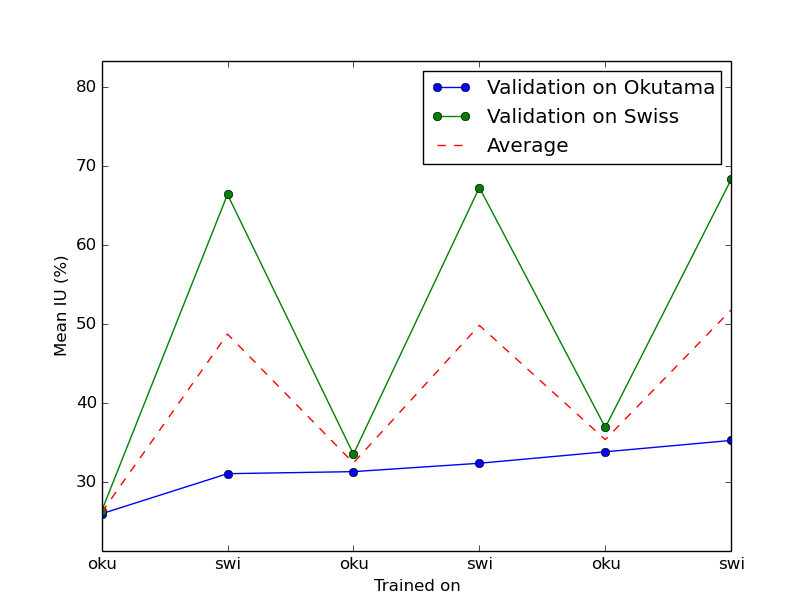
\includegraphics[width=0.8\linewidth,center]{images/part4/ms_1.png}
  \caption{Multi-source trained on baseball field images and improved on Swiss - accuracies over cycle}\textbf{
  \label{fig:part4:ms_1}}
\end{figure}

\item The second training is actually exactly the same as above, but with other data : the source dataset is now the school dataset, and the validation set is composed of the images taken from the baseball field. The Multi-source remains the same, trying to improve the results of the learning on Okutama using the Swiss dataset. The main objective of this experiment is to detect if the images from the baseball field and the ones from the school are "equivalent", that means, if they have similar influence on the learning on Okutama dataset. If we get the same results as above, it would mean that they are equivalent, and that our results are reliable. If we do not, it would mean that one of the two datasets gives more information on the other one than the second dataset on the first one. In this case, we would have to consider the lower result. \\
As shown in the graph~\ref{fig:part4:ms_2}, we notice that the results are  better in this experiment, so we can imagine that the dataset with images taken from the school includes many information concerning images taken from the baseball field. The reciprocal seems false.

\begin{figure}[ht!]
  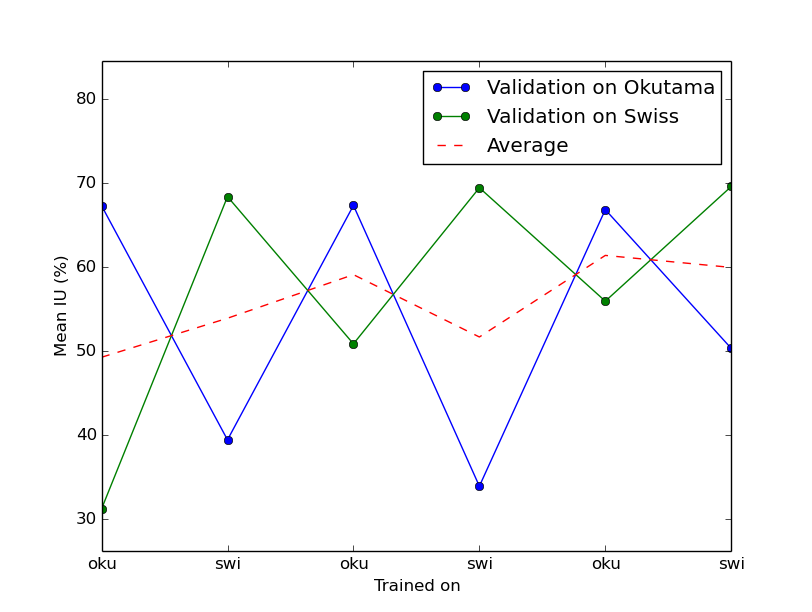
\includegraphics[width=0.8\linewidth,center]{images/part4/ms_2.png}
  \caption{Multi-source trained on school images and improved on Swiss - accuracies over cycle}\textbf{
  \label{fig:part4:ms_2}}
\end{figure}

\item The third experiment is done between the two whole datasets : we first learn features from the Okutama training set (80\%), and try to improve it with the Swiss training set (80\%). The validation set is done on the Okutama and on the Swiss validation sets, we try to improve both of them. \\
This learning shows some improvements on the Swiss dataset, but not a lot on the Okutama set, as seen above, on the first experiment. The graph~\ref{fig:part4:ms_3} shows, again, the evolution of the accuracy. 

\begin{figure}[ht!]
  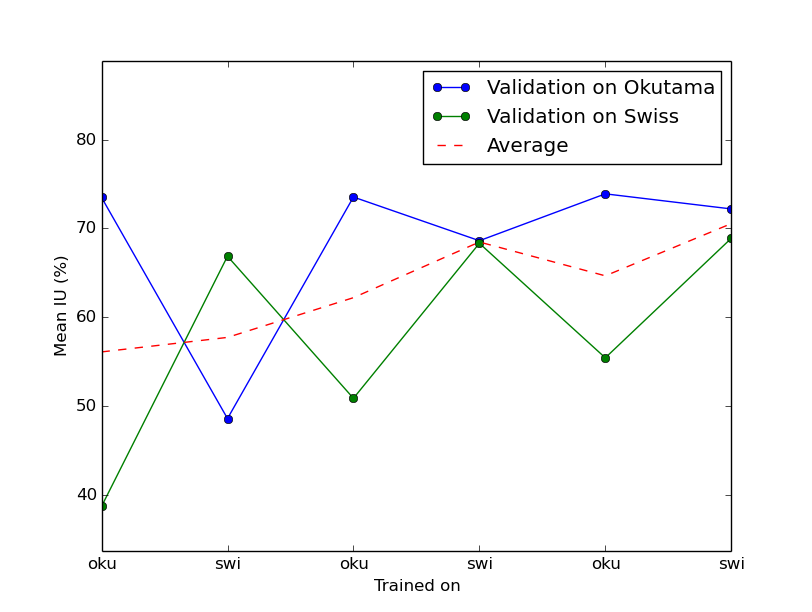
\includegraphics[width=0.8\linewidth,center]{images/part4/ms_3.png}
  \caption{Multi-source trained on Okutama images and improved on Swiss - accuracies over cycle}\textbf{
  \label{fig:part4:ms_3}}
\end{figure}

\end{enumerate}

\subsubsection{The Multi-Source utility}
So it appears that the Multi-Source method shows a real interest for merging efficiently knowledges from two different datasets into one single model, even if it does not improve the accuracy of the source dataset, at least in the case of our datasets. \\
But if we simply want to learn from these two datasets, why would we not simply train our model on all the images all at once ? We also tried this method to compare it with our multi-source method. The table~\ref{fig:part4:setup4} shows the results on both of these experiments, and shows that the accuracies from the multi-source are higher than the ones from the intuitive model. Indeed, the learning with the two different datasets try to learn features suiting to both of them, whereas the multi-source learning try to merge the knowledge on the target dataset into the pre-computed knowledge of the source dataset.

\rowcolors{2}{gray!25}{white}
\begin{table}[htbp]
  \centering
  
  \begin{tabular}{rcccccc}
  \rowcolor{gray!50}
  \toprule
   & \textbf{Train on} & \textbf{Mean IU} & \textbf{fwIU} \\
  \midrule
  Validate on Swiss & both	&		66.68			&	91.76 \\
  Validate on Swiss & ms		&		\textbf{68.87}	&	\textbf{92.52} \\
  \midrule
  Validate on Okutama & both &		68.7	0			&	77.73 \\
  Validate on Okutama & ms   &		\textbf{72.18}	&	\textbf{81.88} \\
  % last two lines switched for results
  \bottomrule
  \end{tabular}%
  
  \caption{Comparison of the data augmentation methods on both datasets.}
  \label{fig:part4:setup4}
\end{table}%

To conclude, multi-source is a good way to learn new models and include them in an other model. If we want to learn how to segment aerial urban views as well as aerial landscape views, for example, multi-source may be one of the best way to do it.


\addcontentsline{toc}{subsection}{Setup 5. Ensembles, efficiency and speed}
\subsection*{Setup 5. Ensembles, efficiency and speed}
Few studies~\cite{MARM16} \todo{find an other one} proves the efficiency of the ensembles method, that means computing few different architectures on the same dataset and, then, averaging their output in a given way. This method is really heavy, and we also need to distillate our result to get a faster (altered) model. The main objective of this part is to see if it is possible to get better results with an altered ensemble than with single models.

The results of our ensembles are shown in the table~\ref{part4:setup5:ensembles}. We can see that we are able to improve our results on our architecture, but it considerably increases the processing time. The table~\ref{part4:setup5:distillated} shows the same ensembles, but with the distillation process which drastically decreases the processing time but also a bit the accuracy. The last table (~\ref{part4:setup5:comp}) simply shows the comparison of the architectures of the ensemble alone with their respective distillated ensembles. It appears that we are not able to improves the accuracy (while keeping the same processing time) using this way, because the distillated ensembles finally appears to provide lower accuracies. Some additional tests may be relevant here, considering that we tried the same technique on an other dataset (Pascal VOC) with success, as shown in the table \todo{add ref} in the appendices.
\todo{redo this table}

\todo{replicate everything}
% from array 1 : 3, 4 are false
% from array 2 : eveything is false
\rowcolors{2}{gray!25}{white}
\begin{table}[ht!]
  
  \begin{subtable}{\textwidth}
    \centering
    \begin{tabular}{cccccc}
    \rowcolor{gray!50}
    \toprule
    \textbf{Name} & \textbf{Mean IU} & \textbf{fwIU} & \textbf{Processing time / img}\\
    \midrule
    1	& 68.43				& 81.13				& 0.37 \\
    2	& 70.41				& 80.11				& 0.37 \\
    3	& \textbf{70.87}		& \textbf{81.15}		& 0.75 \\
    4	& 68.12				& 79.04				& 0.86 \\
    \bottomrule
    \end{tabular}%
    \caption{Experiments for the setup 5 - Ensembles}
    \label{part4:setup5:ensembles}
  \end{subtable}
  
  
  \begin{subtable}{\textwidth}
    \centering
    \begin{tabular}{cccccc}
    \rowcolor{gray!50}
    \toprule
    \textbf{Name} & \textbf{Mean IU} & \textbf{fwIU} & \textbf{Processing time / img} \\
    \midrule
    1	& 66.13				& 78.24				& 0.11 \\
    2	& 69.75				& 78.11				& 0.11 \\
    3	& \textbf{67.02}		& \textbf{80.56}		& 0.12 \\
    4	& 66.62				& 79.04				& 0.11 \\
    \bottomrule
    \end{tabular}%
    \caption{Experiments for the setup 5 - Distillated ensembles}
    \label{part4:setup5:distillated}
  \end{subtable}
  
  \caption{Setup 5}
\end{table}%
\label{part4:setup5}

\todo{add and replicate}
% Everything from distill ens is false
\rowcolors{2}{gray!25}{white}
\begin{table}[htbp]
  \centering
  
  \begin{tabular}{rcccccc}
  \rowcolor{gray!50}
  \toprule
  \textbf{Architecture} & \textbf{Mean IU} & \textbf{fwIU} & \textbf{Processing time / img}\\
  \midrule
  FCN-32-ResNet-50	& 64.90			& 78.0			& 0.11 \\
  FCN-32-ResNet-152	& 67.92			& 80.84			& 0.25 \\
  Distill. ens n°1	& 66.13			& 78.24			& 0.11 \\
  \midrule
  FCN-16-ResNet-50	& 71.10			& \textbf{81.33}	& 0.12 \\
  FCN-16-ResNet-152	& \textbf{72.06}	& \textbf{81.33}	& 0.25 \\
  Distill. ens n°2	& 69.75			& 78.11			& 0.11 \\
  \midrule
  Distill. ens n°3	& 67.02			& 80.56			& 0.12 \\
  \midrule
  FCN-8				& 70.15			& 79.84			& 0.22 \\
  Distill. ens n°4	& 66.62			& 79.04			& 0.11 \\
  \bottomrule
  \end{tabular}%
  \caption{Experiments for the setup 5 - Comparison}
  \label{part4:setup5:comp}

\end{table}%


\section{Final model visualization}
In the previous section, we finally saw many numbers and talked a lot about the accuracy of our models, but we never displayed the visual results.

The figure~\ref{fig:part4:visu_archi} shows some example of the results we get on both datasets for FCN8, FCN-(32/16)-ResNet-152, and with or without data augmentation. We can see, from top to bottom, the improvement of the model accuracy.

\begin{figure}[ht!]
  \centering
  \begin{subfigure}[c]{0.20\textwidth}
    \centering 
  \end{subfigure}
  \begin{subfigure}[c]{0.33\textwidth}
    \centering Swiss
  \end{subfigure}
  \begin{subfigure}[c]{0.45\textwidth}
    \centering Okutama
  \end{subfigure}
  \vspace{0.2cm}
  
  \begin{subfigure}[c]{0.20\textwidth}
    \centering Test samples
  \end{subfigure}
  \begin{subfigure}[c]{0.33\textwidth}
    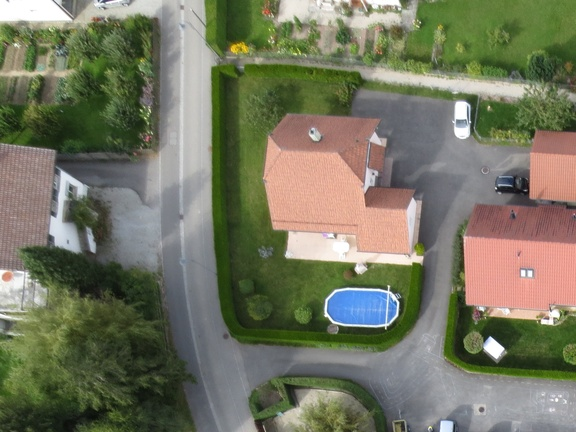
\includegraphics[height=3cm]{images/part4/swi_img.png}
  \end{subfigure}
  \begin{subfigure}[c]{0.45\textwidth}
    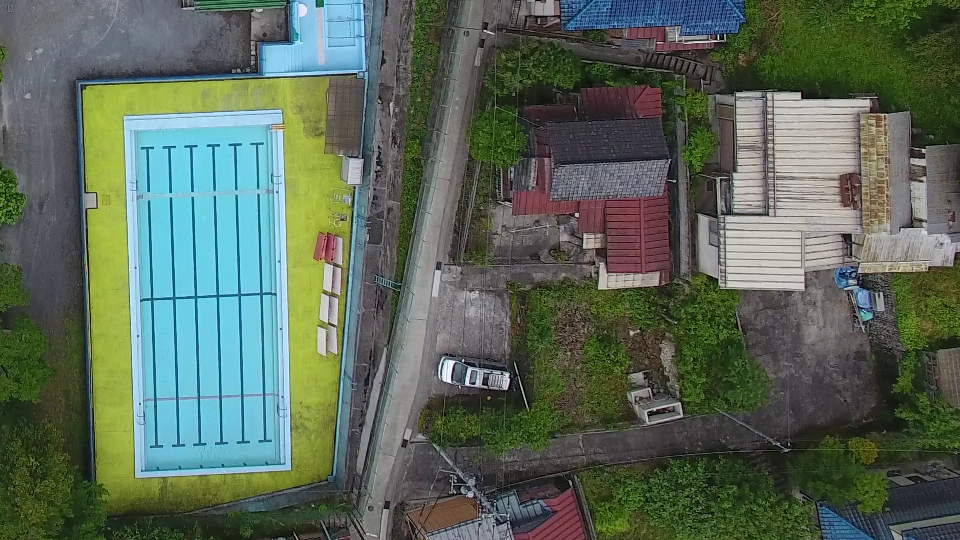
\includegraphics[height=3cm]{images/part4/oku_img.png}
  \end{subfigure}
  \vspace{0.1cm}
  
  \begin{subfigure}[c]{0.20\textwidth}
    \centering Ground truth
  \end{subfigure}
  \begin{subfigure}[c]{0.33\textwidth}
    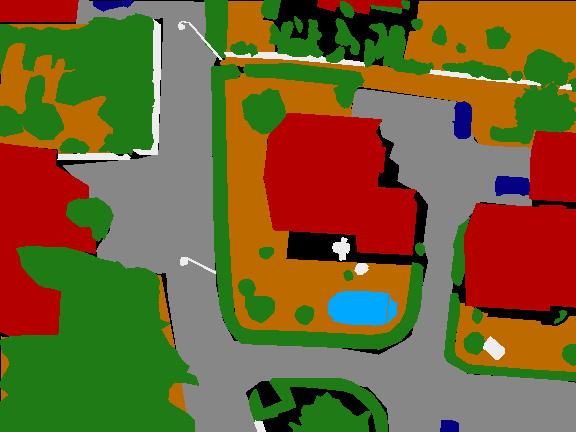
\includegraphics[height=3cm]{images/part4/swi_gt.png}
  \end{subfigure}
  \begin{subfigure}[c]{0.45\textwidth}
    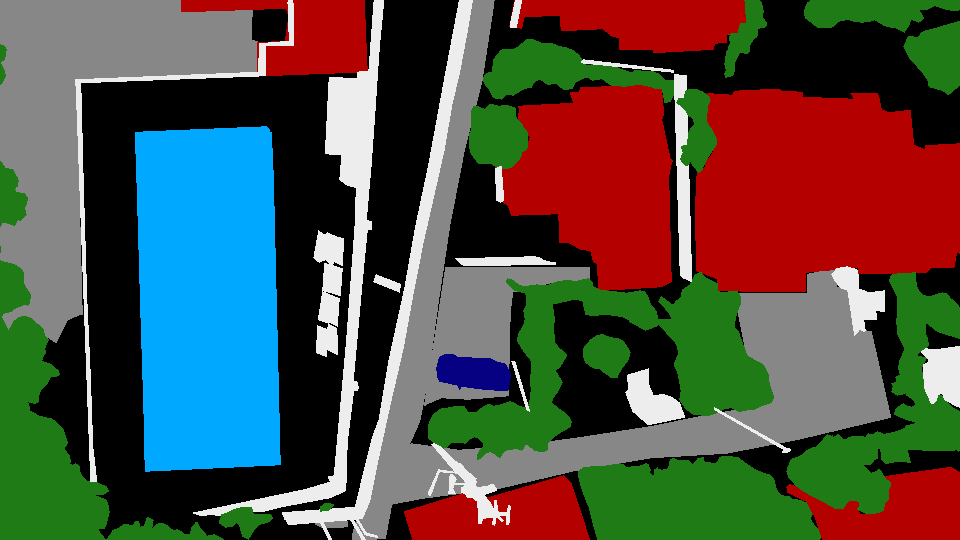
\includegraphics[height=3cm]{images/part4/oku_gt.png}
  \end{subfigure}
  \vspace{0.1cm}
  
  \begin{subfigure}[c]{0.20\textwidth}
    \centering FCN-8
  \end{subfigure}
  \begin{subfigure}[c]{0.33\textwidth}
    
\includegraphics[height=3cm]{images/part4/swi_fcn8.png}
  \end{subfigure}
  \begin{subfigure}[c]{0.45\textwidth}
    
\includegraphics[height=3cm]{images/part4/oku_fcn8.png}
  \end{subfigure}
  \vspace{0.1cm}
  
  \begin{subfigure}[c]{0.20\textwidth}
    \centering FCN-32-ResNet-152
  \end{subfigure}
  \begin{subfigure}[c]{0.33\textwidth}
    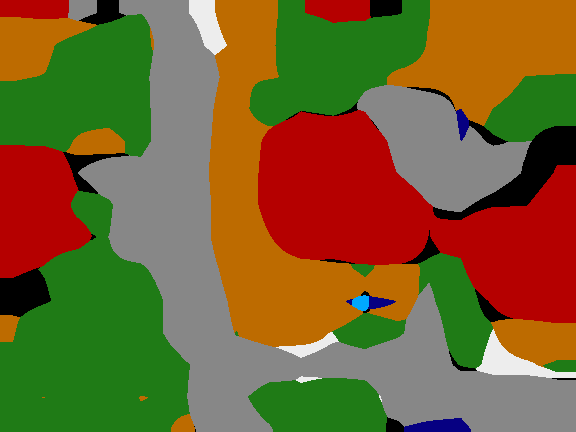
\includegraphics[height=3cm]{images/part4/swi_152.png}
  \end{subfigure}
  \begin{subfigure}[c]{0.45\textwidth}
    
\includegraphics[height=3cm]{images/part4/oku_152.png}
  \end{subfigure}
  \vspace{0.1cm}
  
  \begin{subfigure}[c]{0.20\textwidth}
    \centering FCN-16-ResNet-152
  \end{subfigure}
  \begin{subfigure}[c]{0.33\textwidth}
    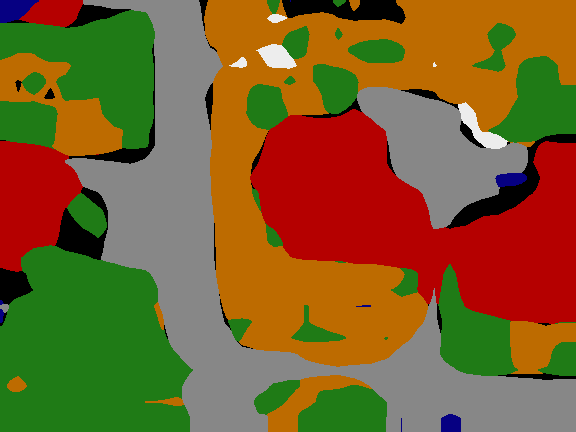
\includegraphics[height=3cm]{images/part4/swi_152s.png}
  \end{subfigure}
  \begin{subfigure}[c]{0.45\textwidth}
    
\includegraphics[height=3cm]{images/part4/oku_152s.png}
  \end{subfigure}
  \vspace{0.1cm}
  
  \begin{subfigure}[c]{0.20\textwidth}
    \centering + Mirror (data augmentation)
  \end{subfigure}
  \begin{subfigure}[c]{0.33\textwidth}
    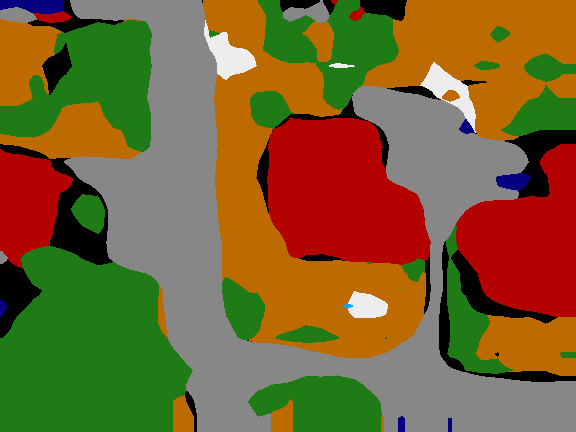
\includegraphics[height=3cm]{images/part4/swi_mirror.png}
  \end{subfigure}
  \begin{subfigure}[c]{0.45\textwidth}
    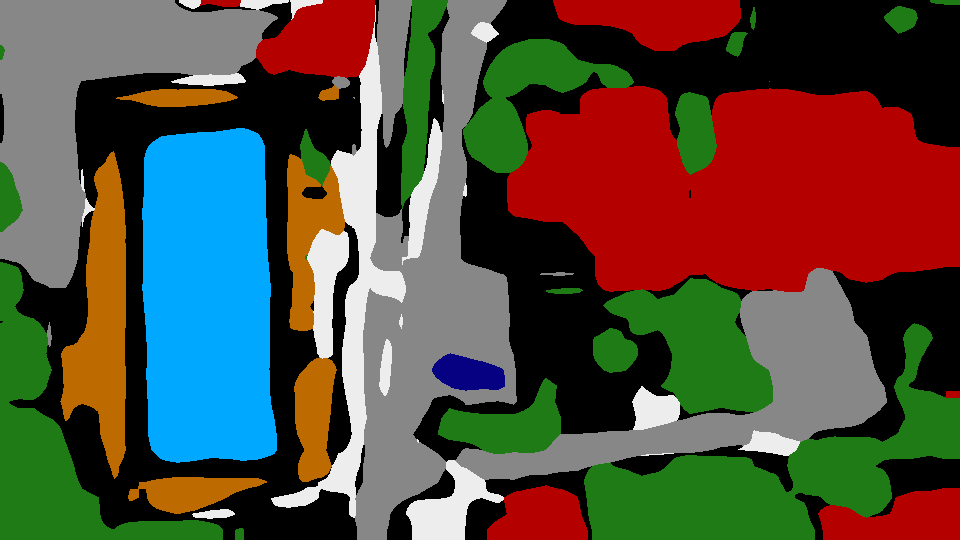
\includegraphics[height=3cm]{images/part4/oku_mirror.png}
  \end{subfigure}
  \vspace{0.1cm}
  
  \caption{Visualization of the performance over architectures and datasets}
\end{figure}
\label{fig:part4:visu_archi}

Also, the figure~\ref{fig:part4:visu_ms} shows an example of the improvement we get using Multi-Source method. This specific example consists in training our architecture on the Okutama dataset and, then, to improve it by training it on the Swiss dataset (last experiment on section~\ref{3:setups:4}). We can clearly see the accuracy improvement on the Swiss validation with the multi-source method, and also can notice that our system is still able to provide a good segmentation on the Okutama dataset. Also, we can compare our segmentations with the segmentations we get by training both datasets all at once, and the multi-source's clearly provide better results.

\begin{figure}[ht!]
  \centering
  \begin{subfigure}[c]{0.20\textwidth}
    \centering 
  \end{subfigure}
  \begin{subfigure}[c]{0.33\textwidth}
    \centering Swiss (Target)
  \end{subfigure}
  \begin{subfigure}[c]{0.45\textwidth}
    \centering Okutama (Source)
  \end{subfigure}
  \vspace{0.2cm}
  
  \begin{subfigure}[c]{0.20\textwidth}
    \centering Test samples
  \end{subfigure}
  \begin{subfigure}[c]{0.33\textwidth}
    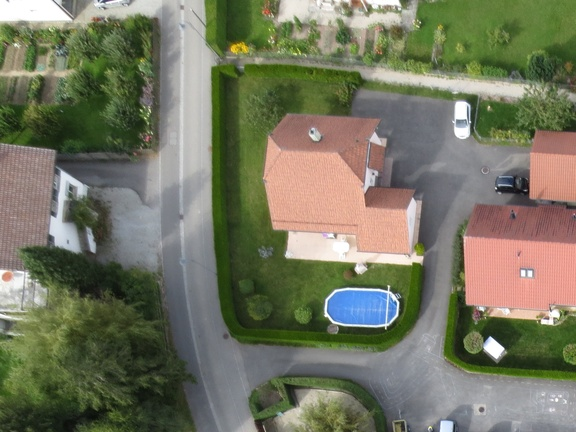
\includegraphics[height=3cm]{images/part4/swi_img.png}
  \end{subfigure}
  \begin{subfigure}[c]{0.45\textwidth}
    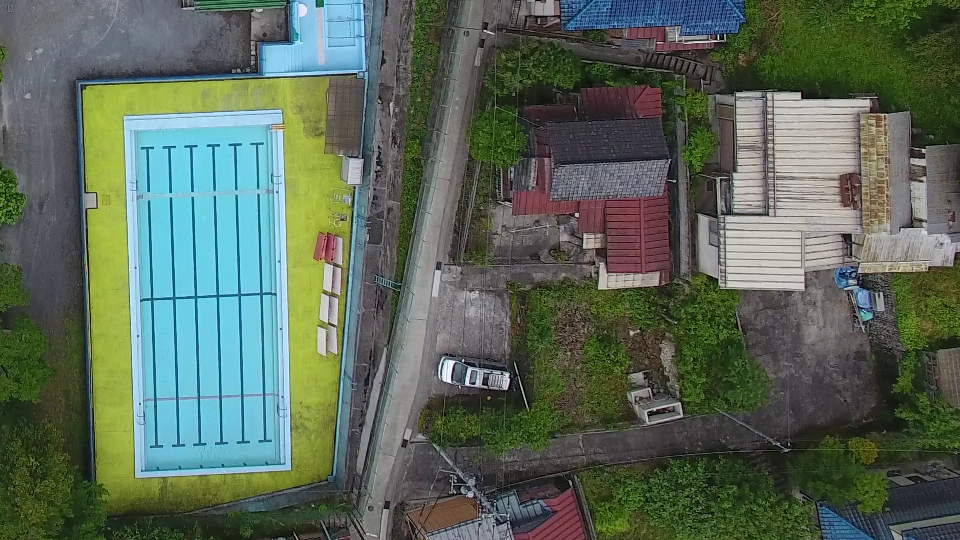
\includegraphics[height=3cm]{images/part4/oku_img.png}
  \end{subfigure}
  \vspace{0.1cm}
  
  \begin{subfigure}[c]{0.20\textwidth}
    \centering Ground truth
  \end{subfigure}
  \begin{subfigure}[c]{0.33\textwidth}
    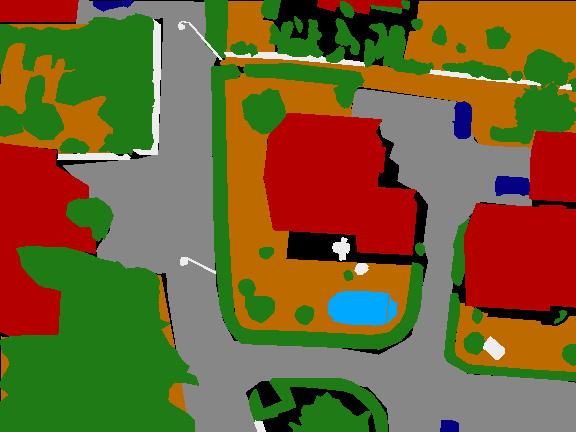
\includegraphics[height=3cm]{images/part4/swi_gt.png}
  \end{subfigure}
  \begin{subfigure}[c]{0.45\textwidth}
    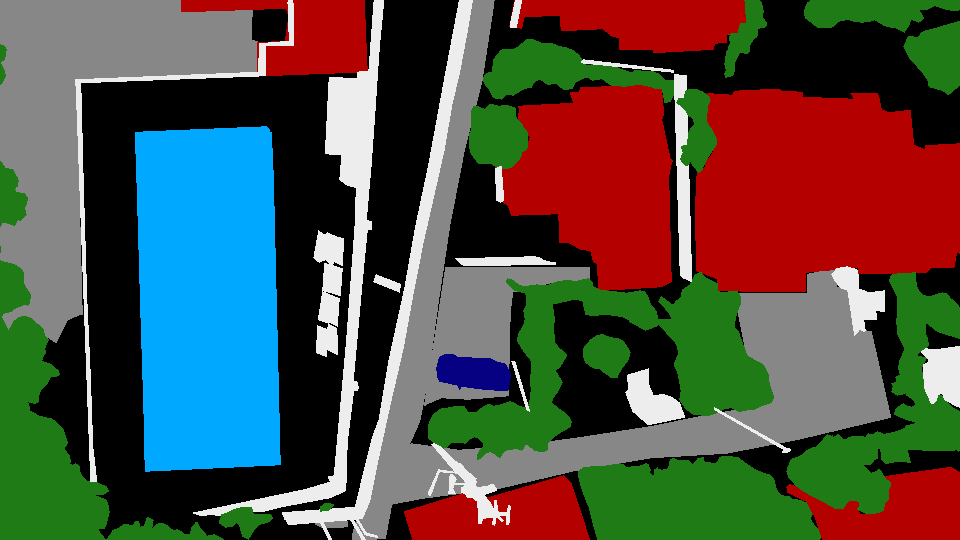
\includegraphics[height=3cm]{images/part4/oku_gt.png}
  \end{subfigure}
  \vspace{0.3cm}
  
  \begin{subfigure}[c]{0.20\textwidth}
    \centering Train both datasets together
  \end{subfigure}
  \begin{subfigure}[c]{0.33\textwidth}
    %\includegraphics[height=3cm]{images/part4/swi_allatonce.png}
    \centering Missing swi\_allatonce.png
  \end{subfigure}
  \begin{subfigure}[c]{0.45\textwidth}
    %\includegraphics[height=3cm]{images/part4/oku_allatonce.png}
    \centering Missing oku\_allatonce.png
  \end{subfigure}
  \vspace{0.3cm}
  
  \begin{subfigure}[c]{0.20\textwidth}
    \centering Train Okutama alone
  \end{subfigure}
  \begin{subfigure}[c]{0.33\textwidth}
    %\includegraphics[height=3cm]{images/part4/swi_okualone.png}
    \centering Missing swi\_okualone.png
  \end{subfigure}
  \begin{subfigure}[c]{0.45\textwidth}
    %\includegraphics[height=3cm]{images/part4/oku_okualone.png}
    \centering Missing oku\_okualone.png
  \end{subfigure}
  \vspace{0.1cm}
  
  \begin{subfigure}[c]{0.20\textwidth}
    \centering Multi-source from Okutama to Swiss
  \end{subfigure}
  \begin{subfigure}[c]{0.33\textwidth}
    %\includegraphics[height=3cm]{images/part4/swi_okutransfered.png}
    \centering Missing swi\_okutransfered.png
  \end{subfigure}
  \begin{subfigure}[c]{0.45\textwidth}
    %\includegraphics[height=3cm]{images/part4/oku_okutransfered.png}
    \centering Missing oku\_okutransfered.png
  \end{subfigure}
  \vspace{0.1cm}
  
  \caption{Visualization of the multi-source method efficiency}
  \label{fig:part4:visu_ms}
\end{figure}

A video example of this work can also be viewed on YouTube, at the following link : https://youtu.be/X73HLjDhtKU.



\section{Test on real device}
We have defined a good architecture for semantic segmentation on aerial views and we, now, want to use it on real situations, that means to implement it in our drone to see if the accuracy and speed would be good enough on a small device (and not anymore on a powerful server).

The implementation will be done on a 64-bit ARM\textregistered A57 CPU, that will run the DL architecture \textit{via} Caffe on the Jetson TX1 GPU~\footnote{nvidia.com/object/jetson-tx1-module}, from Nvidia. These devices are handled by the Phantom drone from DJI~\footnote{dji.com/jp/product/phantom} that captures images of size 3840x2160 with a 4K GoPro.

It appears that the speed of our architecture considerably decreased when it is implemented in the drone : we have a result closer to one frame per second (1FPS) instead of 10FPS on the server. The 1FPS is still acceptable for applications in quite real-time, but would not be enough for more complicated tasks, considering that the understanding of the scene is not everything, we would still want to implement some action algorithms, depending on the understood situations. It may takes some additional time, require a free GPU, and the 1FPS may quickly be a strong limitation.

A first solution would be to process smaller images (ours are high definition, this is quite big and probably not that useful). Cropping the image into a medium field-of-view will accelerate the processing time. Moreover, this operation can be done directly from the camera, to avoid images pre-processing time. However, it also will decrease the understanding of the scene : the drone would segment the really "in front" scene, and would not have a understanding on a large field of view as before.

A second solution would be to optimize our code, currently wrote in Python, and maybe to convert it into C++, which is much weaker. However, we have to admit that our code already use some really optimized libraries (\textit{numpy}, \textit{scipy}, ...), and the conversion of our code into C++ may provide only a slight improvement.

Currently, our project is frozen there, we try to find some other ways to decrease the computational needs on the drone, and to provide a real-time application.



         \pagebreak
  \chapter{Discussion}


At this point, we studied the state-of-the-art, compared few architectures and selected the best one for aerial views. We also tried to improve our results by using data augmentation, deep transfer learning methods, and compressed ensembles. But even considering all of these experiments, the accuracy of our model is still not perfect, we will propose, in this part, few hints that may improve it.


\section{The architecture}
The selected architecture is the ResNet-152 architecture, with the upscaling method from FCN-16. The figure~\ref{fig:part5:fcn16_resnet_architecture} shows its variant with only 50 layers (for the visibility). It has three really notable characteristics : (1) its depth, it is currently one of the architecture with the biggest number of layers, (2) its residual dimension from ResNet, it permits it to dramatically reduces its number of parameters and so, its computational needs and accuracy, and (3) its end-to-end upscaling method, that can be added at the end of any architecture.

\begin{figure}[ht!]
  \includegraphics[width=\linewidth,center]{images/part5/fcn16_resnet_architecture.png}
  \caption{Architecture of FCN-16-ResNet-50}\textbf{
  \label{fig:part5:fcn16_resnet_architecture}}
\end{figure}

The results found in section~\ref{4:setups} proves the efficiency of this architecture, but we still can look for a way to improve it. Few points can be considered :
\begin{itemize}
\item About the depth, as we saw in section~\ref{1:comparison:comparison} last architectures seem to reveal that the more deep it is, the best it is. The only problem seems to come from the number of parameters that a deep architecture involves. But for now, the relation between depth and efficiency is not proven yet : the last architecture from Google is actually not as deep as ResNet (75 layers instead of 152) and provides a slight improvement on ILSVRC challenge.
\item We decided to use the ResNet architecture (which provides the best results on ILSVRC 2015 challenge) with its residual connections. However, it is not proven that these connections are the best way to decrease the total number of parameters. Indeed, Google also proposed its own method, involving inception layers. We may have to try to use them in our aerial views, they may be more efficient.
\item We used the upscaling method from FCN-32 and, then, from FCN-16, that improves the accuracy. We tried, at the really beginning of the project, to create the FCN-8-ResNet-x architecture, and it did not improves the accuracy at this moment. Today, we have a better knowledge on the Deep Learning architectures, and maybe we would be able to implement it "the good way", that would improve our results. Also, we did not really studied the upscaling method from SegNet because it is complicated to implement (not included in the last Caffe version, so we need to re-code the upsampling layers by ourself, which is doable, but not considering the given time for this project). This other upsampling method seemed to give better results than FCN-8 according to its authors and combining it with the residual dimension of ResNet may be interesting.
\end{itemize}



\section{Another DTL method ?}
As we saw, our Deep Transfer Learning was not really efficient for improving a learning : it only permits to merge two knowledges from two datasets into a single one. So, our initial expectation is not reached, and that is a bit disappointed because we also did the same experiment using two different datasets (Pascal VOC and MS COCO) and get better results (results displayed in appendices \todo{add ref}).

Considering this, we can imagine that we may be able to improve our learning by modifying some extra-parameters, like decreasing the learning rate through the cycles of the multi-source process, to reduce progressively the influence of the learnings cycle after cycle.



\section{Post-processing, thinking with videos}
An other idea, that we did not explore at all, would be to process images as part of a video instead of single images, all independent. Indeed, the architectures we saw proved their accuracy \textit{via} computer vision challenges, so they need to focus their segmentation skills on single images. But in our case, we know that we are going to process videos, so we can imagine a new architecture that pre-estimate the output segmentation using the one from the previous image (or images). Indeed, using the few earlier images, it is possible to build trivial object tracking and, then, to improve dramatically the accuracy of a system while applying some pre-probabilities on each pixel of next images. This can be done with multiple technical such as Gaussian numbers, or Bayesian optimization.

Using this kind of implementations, we can expect a significant improvement of the accuracy that may allow us to reduce the complexity of our network. It means that, considering the fact that our accuracy will be corrected by our probabilistic-"tracking" method, we can reduce the complexity of the network by reducing its depth, number of parameters, etc.



\section{Possible applications}
Many applications that would need a semantic segmentation on aerial views are possible and, even if we would not implement any of them in this project, we would list here some possibilities :
\begin{itemize}
\item Suspicious traffic or crowd detection : while flying above a city, a drone can determine if the traffic seems suspicious in comparison with his daily experiences (detection of traffic-jams for example, or manifestations, crowds).
\item Pre-cartography : by knowing what it sees (roads, building, etc), a drone can build a map while flying. Of course, it would only be a first draft, but it can provide a good first idea.
\item Creation of a Dynamic map : as a more ambitious project, we can imagine a drone fleet updating, in real time, a map with its intrinsic information, such as traffic, constructions, works ongoing, special events, ...
\item Intelligent vision for rescue or exploration situation : in an urgent exploration mission, a drone may be able to fly above a dangerous area (post-fire, post-crumbling, ...) and detect irregularities such as human bodies to rescue.
\item Intelligent and flexible delivery by drone : nowadays, drones are able to fly from a point A to B, even with difficult weather conditions or ground irregularities. It can be used for drone deliveries, but, for now, the drone would not be able to fly directly to the message addressee : it would go exactly to the given GPS position. Semantic segmentation may be able to fix this and provide delivery hands to hands.
\end{itemize}



         \pagebreak
  
  \bookmarksetup{startatroot}
  \chapter*{Conclusion}
\addcontentsline{toc}{section}{Conclusion}


Conclusion
         \pagebreak
  \bibliographystyle{abbrv}
  \bibliography{bibli}
  \begin{appendices}

\begin{figure}[!h]
  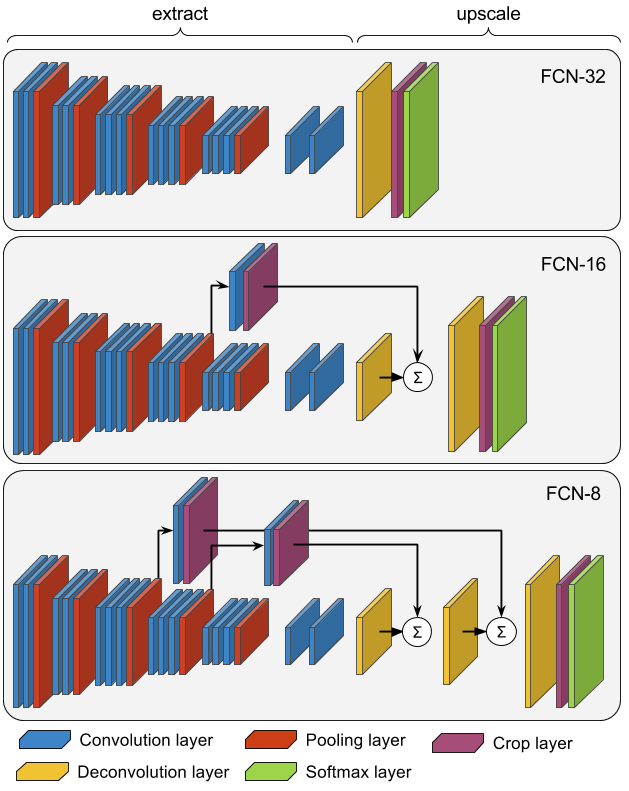
\includegraphics[width=1\linewidth,center]{images/appendices/fcns_architecture.png}
  \caption{Comparison of the three architectures of FCN}\textbf{
  \label{fig:appendices:fcns_architecture}}
\end{figure}

\todo{create with subfigures}
\begin{figure}[!h]
  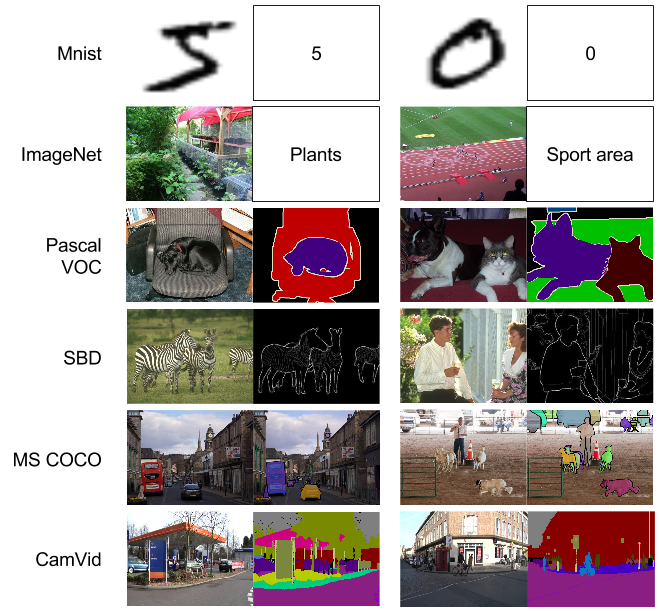
\includegraphics[width=1\linewidth,center]{images/appendices/datasets_comparison.png}
  \caption{Comparison of the most famous datasets}\textbf{
  \label{fig:appendices:datasets_comparison}}
\end{figure}

\begin{landscape}
\begin{table}[htbp]
  \centering
  \begin{tabular}{rcccccc}
    \rowcolor{gray!50}
    \toprule
    yop & yop & \textbf{Caffe~\footnote{caffe.berkeleyvision.org} Berkeley} & \textbf{CNTK~\footnote{cntk.ai} Microsoft} & \textbf{Tensorflow~\footnote{tensorflow.org} Google} & \textbf{Theano~\footnote{deeplearning.net/software/theano} Montreal Univ} & \textbf{Torch~\footnote{torch.ch} N.Y.U} \\
    \midrule
    Available pre-trained models (CNN) & LeNet  & V & X & X & V & V \\
    yop & AlexNet  & V & X & X & V & V \\
    yop & VGGs  & V & V & V & V & V \\
    yop & GoogleNet  & V & X & X & V & V \\
    yop & ResNet  & V & X & X & X & X \\
    yop  & SegNet  & V (C) & X & X & X & X \\
    yop  & FCNs  & V & X & X & X & X \\
    Speed (one GPU) & yop  & Fast & Fast & Slow & Fast & Very fast \\
    Number max of GPU & yop  & 4 & 8 & 4 & 2 & 2 \\
    CudNN compatibility & yop  & V & V & V & V & V \\
    Modelling capability & CNN & V & V & V & V & V \\
    yop & RNN & X & V & V & V & X \\
    yop & New models & X & V & V & V & V \\
    Readable source code & yop & V & X & X & X & V \\
    Interface & yop & Command line (pycaffe) & Command line & Python, C++ & Python & Lua \\
    Architecture & yop & Rigid & Quite modulable & Clean and modulable & Modulable but not intuitive & Clean and modulable \\
    \bottomrule
  \end{tabular}%
  
  \caption{Frameworks comparison}
  \label{appendices:frameworks_comparison}
\end{table}%
\end{landscape}

\todo{to complete}
\rowcolors{2}{gray!25}{white}
\begin{table}[htbp]
  \centering
  
  \begin{tabular}{rcccccc}
    \rowcolor{gray!50}
    \toprule
    \textbf{Architecture} & \textbf{Mean IU} & \textbf{fwIU} \\
    \midrule
    SegNet &				xx & 		xx \\
    FCN-32 &				xx & 		xx \\
    FCN-32-16 &			xx & 		xx \\
    FCN-32-16-8 &		xx & 		xx \\
    FCN-32-ResNet-50 &	xx & 		xx \\
    FCN-32-ResNet-101 &	xx & 		xx \\
    FCN-32-ResNet-152 &	xx & 		xx \\
    FCN-16-ResNet-50 &	xx & 		xx \\
    FCN-16-ResNet-101 &	xx & 		xx \\
    FCN-16-ResNet-152 &	xx & 		xx \\
    \bottomrule
  \end{tabular}%
  
  \caption{Comparison of the accuracy of different architectures on the Okutama dataset}
  \label{appendices:setup2:_oku}
\end{table}%


\end{appendices}
\end{document}

